% Note: To remove the "DRAFT VERSION" warnings, replace the following line with:
% \documentclass[final]{cubedoc}
\documentclass[final]{cubedoc}

\title{A short thermal properties journey for the PCB/package level} %% Assignment Title
\docid{AcubeSAT-THE-BH-032}

\author{Theodoros Katzalis}

\changelog{15/04/2020}{0.1}{DRAFT}{Initial revision}
\changelog{15/04/2020}{0.2}{INTERNALLY RELEASED}{First release}
\changelog{18/08/2020}{0.3}{INTERNALLY RELEASED}{Updated:
	\begin{itemize}
		\item Fix typos.
		\item Table \ref{tab:plate}: Heat Capacity of Tin changed from 0.226 to 226.
	\end{itemize}
	\bigskip
	
	Added:
	\begin{itemize}
		\item Tables \ref{fig:tab_1}, \ref{fig:tab_2}
		, \ref{fig:tab_3}, \ref{fig:tab_4}.
		\item Footnote for .bxl extension.
		\item Image sources and archive websites.
	\end{itemize}
}

\usepackage{tablefootnote}
\usepackage{longtable}
\usepackage{multirow}
\usepackage{supertabular}
\usepackage{adjustbox}
%\usepackage{indentfirst}
\usepackage{subcaption}
\usepackage{graphicx}
\usepackage{hyperref}
\usepackage{cleveref}


%\hypersetup{
%    colorlinks=true,
%    urlcolor=blue,
%    linkcolor=black,
%    citecolor=black
%}


\begin{document}
	
	\section{Introduction}
	
	This is a \textbf{summary} report for the research about thermal properties of the materials used for AcubeSAT's PCBs. A bunch of resources, documentation and issues are listed because during the process some conflicts and uncertainties emerged. I should mention, also, that thermal analysis is very demanding and complex topic, so the documentation of the sources and thinking-paths are valuable tools to spot the possible wrong assumptions and \textbf{fallacies}. \textbf{The until now estimating values for this research can be found in \href{https://drive.google.com/open?id=1gGPhBZe94Yt7D8FDdGNza4ZnG0pRfhT0xG7Z2tBdK7o}{this} spreadsheet}.
	
	%Say that in the LQFP section we will make a more detailed analysis from the rest of the packages. But what is packaging and what is the LQFP thing?
	
	
	%\section{Encapsulation}
	
	%Mold compounds are the materials used for the IC packaging aka the encapsulation. Mold compounds are composite materials. They referred mostly as epoxy mold compounds (EMC) and most of the times the epoxy cresol novolac or the bisphenol something as epoxy resins are used. There are some references scattered around for the thermal properties but they may differ because each supplier using its own recipe. 
	
	\section{Electronic packaging}
	
	There are many reference points that the electrical components can be grouped. The most common one is based on how they interconnect with the PCB. If holes should be used, then we are using the through hole technology (\textbf{THT}) and if the device is mounted, then we are using the surface mount technology (\textbf{SMT}). The devices that are using the last one, as an interconnection method, are called SMDs and they can be divided to many categories too. For now, we will divide them to the \textbf{leaded} and the \textbf{leadless}. In the first belong the packages that their leads extend beyond the package and in the second when they don't. We are going to focus in the SMDs because if not everything, almost all the components that are going to be used in the AcubeSAT's boards, except the PC104 connectors, will use the SMT. 
	
	Before diving into what is hidden under the hood of the black boxes that we are looking in the PCB, we need first to demystify the terminology. \textbf{Packaging} is an abstract word and is used a lot in the electronics but it has several meanings and "thought layers". There are the chip packaging, the PCB packaging and the systems packaging where a lot of PCBs are interconnected with each other. In a different way, packaging can be referred to \textbf{integrated circuit} and \textbf{electronic}. Electronic packaging has to do with everything about the interconnection of the die with the external circuitry of a PCB. The integrated circuit packaging is actually the last step of the electronic one. It is referred to the encapsulation process, the protection of the IC from the rest of the environment.
	
	But lets stay more in the electronic packaging definition. There are four main levels:
	
	\begin{enumerate}
		\item \textbf{Semiconductor} (or die, chip, IC) level. The wafer is separated into chips and one of them is inside of the package. The die, most of the times, is Si based, but GaAs can be used for high speed applications. In the die level, metalization (Al, Cu, Ag) takes place for oxidation protection.
		\item \textbf{Chip in a carrier}. This is where all the bonding takes place. The die is attached to a leadframe or a substrate  and the wire bonds serve the role of interfacing the integrated circuit with the outer leads (these terms will be explained soon). For the die attachment we have conductive or non conductive adhesive (but always thermal conductive) . If there is an exposed pad for example and electrical connection is desired, then the first one is used\footnote{Most of the times the exposed pad will be grounded but you need to be sure checking the datasheet otherwise problems may occur.}. 
		\item \textbf{PCB level}. The chip is mounted on the board either with leads or no leads. Then the leads via copper tracks are connected with other components.
		\item \textbf{System level}, PCB to PCB interconnect. This is where multiple PCBs are connected all together for a large application.
	\end{enumerate}
	
	In order to understand a little bit more all of these new/fuzzy terms like die, leadframe, substrate, wirebonds (bonding-wires), we will give an example of a package based on the through-hole technology. Thus let's take a look of a very well-known package that showed among the first ones in the job market. This is the dual line package (\textbf{DIP}). As we can see, the leadframe is the structure that houses the chip and interfaces the integrated circuit with the leads. The interface that change the pitch from the die to the outer leads is called \textbf{interposer}. Sometimes leadframe and interposer are used interchangeably. The materials used in the leadframe is copper or copper alloys and it is usually plated with tin or gold over nickel for oxidation-protection and to ensure wirebondability and solderability for the assembly process. The die is attached to the leadframe pad using an organic compound (die attachment), epoxy resin with metal fillers (e.g. silver). Finally, for the encapsulation, the most used and cost-effective solution is the plastic package. It is epoxy resin with ceramic fillers like fused silica or alumina. It should be noted that \textbf{mold compounds} are called the materials used in the encapsulation process. 
	
	%Add the thermosetting property of the plastic thing, temperature and the moling process and the polymeric, adhesive nature and so on???????//
	
	\begin{figure}[h!]
		\centering
		\begin{subfigure}{.5\textwidth}
			\centering
			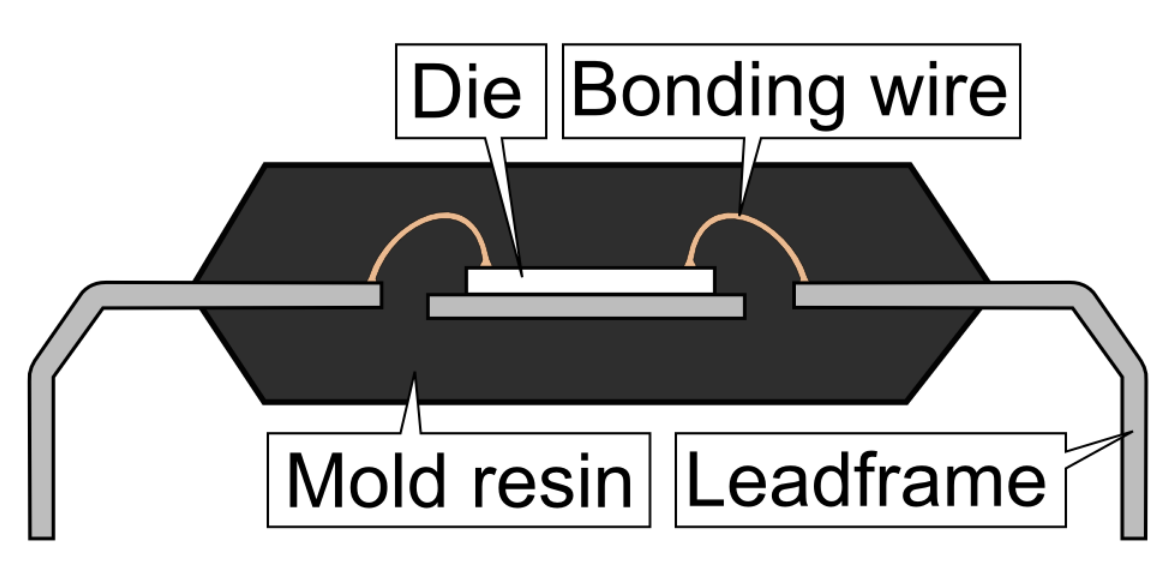
\includegraphics[width=0.7\linewidth]{docs/pdip.png}
			\caption{DIP cross section view \small{(\href{https://web.archive.org/web/20200818152711/https://commons.wikimedia.org/w/index.php?title=File:DIP_package_sideview.PNG&oldid=131332920}{image source})}}
			\label{fig:sub1}
		\end{subfigure}%
		\begin{subfigure}{.5\textwidth}
			\centering
			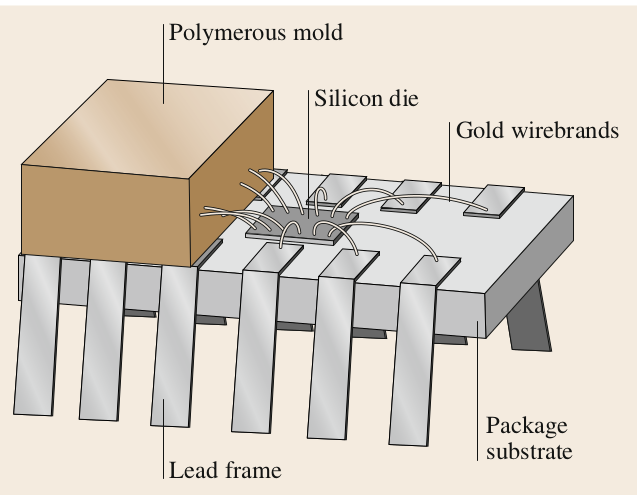
\includegraphics[keepaspectratio, width=0.7\linewidth, height=.4\textheight]{docs/dip_leadframe.png}
			\caption{DIP leadframe \small{(\href{https://web.archive.org/web/20200818152844/https://link.springer.com/chapter/10.1007/978-3-319-48933-9_530}{image source})}}
			\label{fig:sub2}
		\end{subfigure}
		\caption{}
		\label{fig:test}
	\end{figure}
	
	The DIP package that we have mentioned belongs to the plastic leadframe-based packages. That implies that the IC packaging can be, for once more, categorized in terms of material packaging to the \textbf{plastic and ceramic} ones and in terms of housing/supporting the die to the \textbf{leadframe and the substrate}.
	
	For the difference between the ceramic and the plastic we are going to use the Cer-DIP as an example. Yes you guess right, it is a DIP but with ceramic materials for the packaging. So, a typical ceramic package has a ceramic base/leadframe that is embedded to glass and a lid. The ceramic material that is used most often is the Aluminum oxide (alumina) and for the lid, metal or ceramic ones. The benefits of ceramic packaging is the hermetic feature, the increased reliability and the greater thermal conductivity (one order of magnitude more) than plastic polymeric epoxy resin based packages. The main drawback is the cost and thus it is avoided for mass production. 
	
	%Say that in general ceramic and plastic are bad but ceramic is better. It is difficult to be an insulator and at the same time thermal conductive but with composite and compound material is somehow achievable! It is a challenge. But the detailed thermal characterisitcs I will write them in the LQFP section. I dont know where to put the saltsa for every topic. I have a lot of abstract. I will maybe put them in the inroduction section but it will miss the point of the thermal properties. I mean lets write for the packages, the dimension and the soldering paste, the plating and so on.
	
	\begin{figure}[h!]
		\centering
		\begin{subfigure}{.5\textwidth}
			\centering
			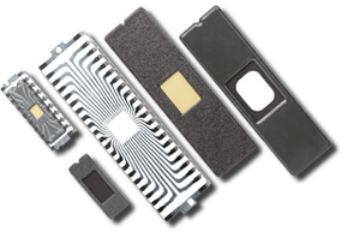
\includegraphics[height=0.2\textheight, width=\textwidth, keepaspectratio]{docs/cer_dip_real.png}
			\caption{Three main parts of a CER-DIP: base,\\ 
				leadframe, lid  \small{(\href{https://web.archive.org/web/20200818153119/https://www.spectrum-semi.com/cerdip}{image source}})}
			\label{fig:sub1}
		\end{subfigure}%
		\begin{subfigure}{.5\textwidth}
			\centering
			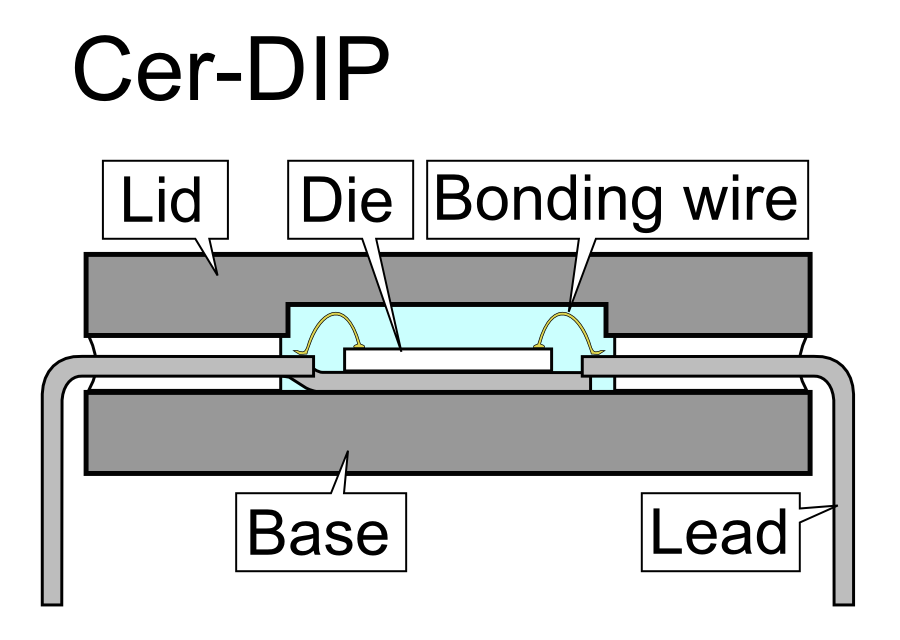
\includegraphics[height=0.2\textheight, width=\textwidth, keepaspectratio]{docs/cdip.PNG}
			\caption{Cross section view of a ceramic package \small{(\href{https://web.archive.org/web/20200818153102/https://commons.wikimedia.org/wiki/File:Cer-DIP_package_sideview.PNG}{image source})}}
			\label{fig:sub2}
		\end{subfigure}
		\caption{}
		\label{fig:test}
	\end{figure}
	
	Before proceeding further, for one more time we will make another division and we will describe the leadframe-based and the substrate packages.
	For the leadframe style we have mentioned the DIP, but what about the substrate-style? So to understand this, we will make a huge jump and we will move to a more advanced packaging method, to the family of grid array and more specific to the Land Grid Array (\textbf{LGA}). In this category is included the component RFFM6406 UHF TX-RX of the communication subsystem so it is sure worth describing, or I should say scratching the surface of this type. A general cross view of a LGA is like this (Figure \ref{fig:sub2}). The die is now glued, instead of a leadframe, to a substrate that is actually a laminate that is like a PCB! So we have a "PCB inside a PCB". It may have a lot of copper and dielectric layers along with soldermask to the top. The die is attached to the top layer. Then the wirebonds are attached to some exposed copper areas of the top layer and with vias the integrated circuit is now connected to the exposed pads in the bottom surface that serve the interface of the die with the rest of the circuit. This type of packages are used in demanding applications for high speed signals that its thermal and electrical performance is crucial and for populated areas with no room to breathe due to the small size but the increased functionality! 
	
	
	\begin{figure}[h!]
		\centering
		\begin{subfigure}{.3\textwidth}
			\centering
			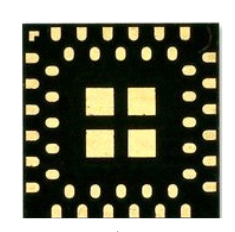
\includegraphics[keepaspectratio, height=.4\textheight, width=\textwidth]{docs/lga.png}
			\caption{Bottom side \small{(\href{https://web.archive.org/web/20200818134018/https://www.nxp.com/docs/en/application-note/AN2265.pdf}{image source})}}
			\label{fig:sub1}
		\end{subfigure}%
		\begin{subfigure}{.6\textwidth}
			\centering
			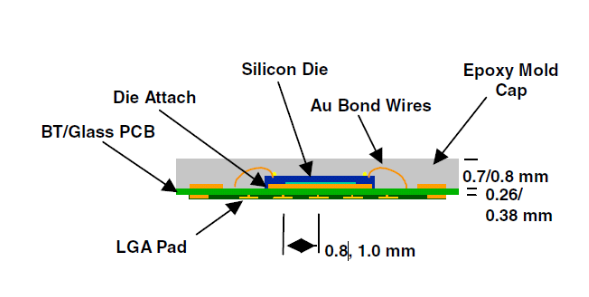
\includegraphics[keepaspectratio, width=\textwidth, height=.6\textheight]{docs/lga_cross.png}
			\caption{Cross section view \small{(\href{https://web.archive.org/web/20200818134018/https://www.nxp.com/docs/en/application-note/AN2265.pdf}{image source})}}
			\label{fig:sub2}
		\end{subfigure}
		\caption{LGA}
		\label{fig:test}
	\end{figure}
	
	%should I talk about the plating and where. We will talk about plating when we are going to see the lead-paste-pcb stuff with the stencil thickness and so on!
	
	%the whole concept that the OBDH MCU will be my test thing to illustrate everything we learned and before diving we will give an overview to familiarize with the terms!!! So about the process ing you could say oven and high temperatures that bond the stuff and the curing and the epoxy, but not detail and proeprties. All of these fun stuff will be lay down right now in the OBDH. So backle up we are starting....
	
	
	%A general view of the ICs. Lead frames, substrates and the list of IC packages along with some materials used. After we are going to use the OBC MCU and we are going to examine the package and the material declaration thoroughly. 
	
	%Now that we have an overview of the packaging, we are going to use the \textbf{OBDH MCU} as an example to check thoroughly the whole packaging thing from the materials point of view and the thermal properties along with the physical dimensions and mechanical drawings. Actually I want to say more about this. Change of plans. We are going to document all the different package of interest
	
	Now that we have an \textbf{overview} of the packaging and the terminology, we are going to examine the packages of the components of the AcubeSAT's board that we assume as critical from a thermal's point of view. The list of these can be found in the aforementioned spreadsheet\footnote{This report may be outdated in the long run if more packages are going to be added}. It should be noted that the following analysis of the IC packages isn't complete and it isn't oriented for a detailed 3D IC simulation. The goal is to find out if we need to create eventually these kind of detailed models based to the materials and their thermal properties that will be listed in the continue of this report. So if eventually a more detailed approach  is necessary, thorough investigation should be made for the standardized dimensions of the internal structure of each package. 
	
	It should be noted that the \textbf{material declaration}, the document that lists all the materials used in packaging, isn't provided for all of them. To be more specific this particular type of doc is successfully indexed from manufacturers such as ST Microelectronics, Texas Instruments (TI) and Analog Devices that generally have great documentation and support. For the rest, by the code-name\footnote{The IC package naming convention is a function of the physical dimensions, pins, pitch and the overall anatomy of the package. Most of them are standardized but vendors may use different names} of the package (e.g. QFP, SOIC), we can safely think abstractly for the anatomy and the materials used. This is not accurate, but it bares the risk for the scope of this report. In other words, if the package is a well known and among the standardized ones, there are many chances that will be identical with other references that using the same package (of course some details may be different). For these with the missing material declaration, if we are finally going to follow the detailed approach, we need, except the standardized dimensions, to contact the vendor and request more information (it is worth mentioning that this kind of contact may be unsuccessful, so a more "delicate" approach would be more suitable). 
	
	Finally, about the approach that we are going to follow, for the physical dimensions part, of the upcoming IC packages, we will focus more to the thermal desired lead-PCB interconnection.
	
	%A word about packages? Plastic and ceramic? Actually the hollistic approach I will put here in this section for alternatives sticked to the DIP package. In the LQFP we are going to stick to the leadframe, the thermal characteristics and so on. Or no? I will think it about after a break! Explain the leadframe and th substrate style and say that OBDH MCU leadframe examined analysis and so. All the other are pretty much the same! I dont know for some reason for the electrical components I have a biased opinion of what should be analyzed first.
	
	\subsection{LQFP}
	
	%The package of the OBDH MCU is called LQFP and this is actually a code-name that is associated with certain physical dimensions (to find out a detailed list of the ic packages with their physical dimensions see here). This type of package is used for other components of the AcubeSAT's boards so the analysis will be sort of the same with all the components under the LQFP umbrella term (and this also applies for each different package that we are going to analyze). But it should be noted that the code-name of the package isn't always associated with a specific material declaration. Each manufacturer have its own recipe so some details may be different. But in general most of the times we can safely assume the type of the package and type of the housing of the die (leadframe or substrate). But if it assumed that we need to test the IC in a detail, then we need sure to contact each manufacturer to provide us the material declaration and the standard for the physical dimensions of the die, die attachment, leadframe, wirebonds and so on. (For now we will continue) We are going to stick to the OBDH MCU though, because it is very well documented from the provider/vendor (st microelectronics) and the material declaration doc, that is necessary to find out the materials used and its thermal properties , is among the documentation, too. 
	
	LQFP stands for Low profile Quad Flat Package, it has 144 pins and it belongs to the very well-know QFP series. There are slight variations for the physical dimensions of the components associated with this code-name, but the AcubeSAT's components with this tag are all the same. These are the \textbf{OBDH, SU and ADCS MCU}.
	%We should mention that we for the physical dimensions part we will focus to the leads-PCB interconnection. So without further ado let's start dissecting this package. Double check that the dimensions are the same.
	
	First, from the material declaration (see the complete document \href{https://web.archive.org/web/20200818131830/https://www.st.com/content/ccc/resource/quality_and_reliability/quality_certificate/material_declaration/group3/be/7d/54/2a/11/68/4e/ad/DM00442253/files/P41A_470XXXY_signed.pdf/jcr:content/translations/en.P41A_470XXXY_signed.pdf}{here}) we can validate that it is a plastic leadframe-based package. But let's make a summary for the listed-materials.
	
	%Oh god, I need to create a table??
	
	\begin{table}[h!]
		\centering
		%\tablehead{\hline}
		%\tabletail{\hline}
		%\tablecaption{Summary of the material declaration of LQFP package}
		\begin{tabular}{ |c|c|c| }
			\hline
			\multirow{1} {*} {\textbf{Parts}} & \textbf{Material} & \textbf{Mass} \\  
			\hline
			\multirow{8} {*} {Die}  & Silicon & 24.184 \\ \cline{2-3} & Aluminum & 0.045 \\ \cline{2-3} & Copper & 0.397 \\ \cline{2-3} & Cobalt & 0.001 \\ \cline{2-3} & Tantalum & 0.129 \\ \cline{2-3} & Titanium & 0.005 \\ \cline{2-3} & Tungsten & 0.003 \\ \cline{2-3} & Silicon Nitride & 0.101 \\ \cline{2-3} & Silicon Oxide & 0.257  \\
			\hline
			\multirow{4} {*} {Leadframe base}  & Copper & 233.880 \\ \cline{2-3} & Iron & 5.760 \\ \cline{2-3} & Zinc & 0.288 \\ \cline{2-3} & Metallic Phosphorous & 0.072 \\ 
			\hline
			\multirow{3} {*} {Leadframe plating}  & Nickel & 9.021 \\ \cline{2-3} & Palladium & 0.140 \\ \cline{2-3} & Gold & 0.140 \\ 
			\hline
			\multirow{7} {*} {Die attachment}  & Copper & 2.170 \\ \cline{2-3} & Iron & 0.155 \\ \cline{2-3} & Silica fused & 0.310 \\ \cline{2-3} & Metallic Phosphorous & 0.016 \\ \cline{2-3} & Diluent & 0.155 \\ \cline{2-3} & Allyl Compound & 0.155 \\ \cline{2-3} & Hardener & 0.140 \\
			\hline
			\multirow{4} {*} {Bonding wires}  & Gold & 2.376 \\ \cline{2-3} & Palladium & 0.024 \\ \cline{2-3} & Silver & 0.000 \\ \cline{2-3} & Copper & 0.000 \\
			\hline
			\multirow{6} {*} {Encapsulation}  & Epoxy resin A & 20.706 \\ \cline{2-3} & Epoxy resin B & 41.412 \\ \cline{2-3} & Silica Amorphous A & 811.789 \\ \cline{2-3} & Silica Amorphous B & 88.001 \\ \cline{2-3} & Carbon Black & 5.177 \\ \cline{2-3} & Phenol resin & 67.295 \\
			\hline
			\multirow{3} {*} {Finishing}  & Nickel & 0.679 \\ \cline{2-3} & Palladium & 0.011 \\ \cline{2-3} & Gold & 0.011 \\ 
			\hline
		\end{tabular}
		\caption{Material declatation OBC MCU}
		\label{tab:matdoc}
	\end{table}
	
	
	As we can see in the table \ref{tab:matdoc}. in the die level the base material is the Silicon and all the other metals are used for the so called metallization that serves the role of oxidation protection for the chip. The die attachment is a typical epoxy resin with silver as filler metal and for the leadframe we have a copper alloy that it is pre-plated with nickel over gold.
	
	%A talk about die attachment, a talk about bonding wires and talk about mold compounds, the organic materials and so on!! And redirect here for more info and say in general that for the lqfp more information and alternatives will be added and some concerns. I will figure it out. Now thermal proeprties, the ultimate table. Say here that other used materials could be such and such, and that in the material declaration the gold choice is among the popular ones and this type of writing. A little more details about what else could be the materials and thei role for protection and oxidation. Not too much though
	
	\begin{figure}[h!]
		\centering
		\begin{subfigure}{.5\textwidth}
			\centering
			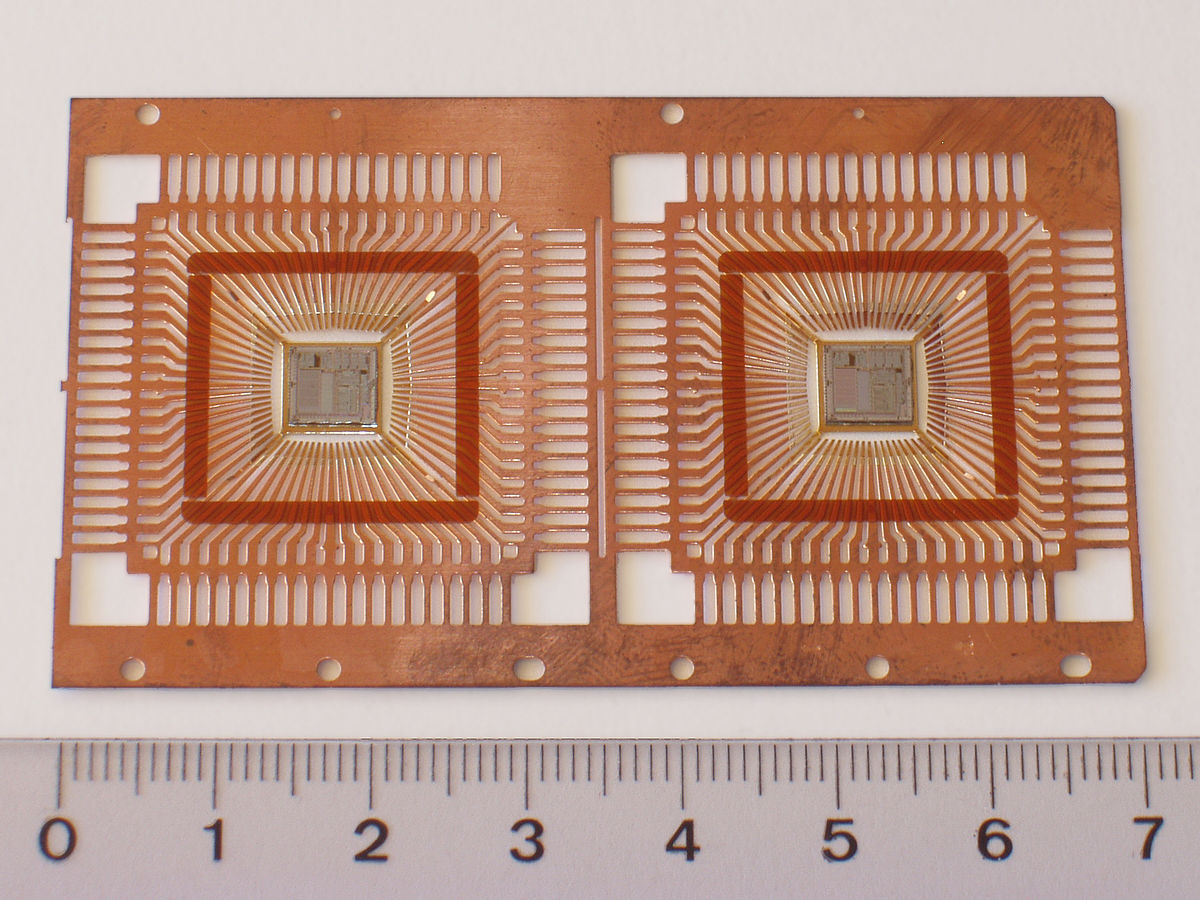
\includegraphics[keepaspectratio, width=0.7\linewidth]{docs/leadframe_qfp.jpg}
			\caption{Two QFP leadframes \small{(\href{https://web.archive.org/web/20200818153249/https://commons.wikimedia.org/wiki/File:TQFP_Leadframe.jpg}{image source})}}
			\label{fig:sub1}
		\end{subfigure}%
		\begin{subfigure}{.5\textwidth}
			\centering
			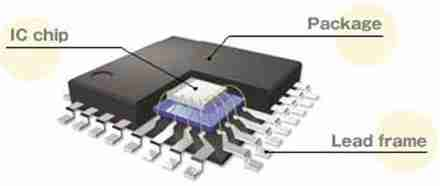
\includegraphics[keepaspectratio, width=\linewidth, height=.6\textheight]{docs/qfp_anatomy.jpg}
			\caption{QFP package anatomy \small{\href{https://web.archive.org/web/20200818153744/http://resource.renesas.com/lib/eng/fab/index.html}{image source}}}
			\label{fig:sub2}
		\end{subfigure}
		\caption{}
		\label{fig:test}
	\end{figure}
	
	\subsubsection{Thermal properties}
	%Actually it would be bloated if I say too much for the alternatives and so on. I will just add some few words more in the above paragraph
	
	%I will create a list of tables and there I am going to put all the references. We need data for the encapsulation the most and the leads. Copper electroplated!!
	
	%One major problem where are the tables for the thermal properties? I need to make an overall assesment of the materials. Then I need to recall why some materials are used just for the sake of completeness. Then the rest will be pretty much easier. Theta values will be a little bit hard probably!! But we can handle it, no worries!! We found awesome package application note for all the leaded packages from infineon too!!
	
	About the thermal properties, an all in one solution for the requested ones (thermal conductivity, heat capacity, absorptivity, emissivity) couldn't be indexed. Instead a lot of references have been found scattered around the web. Of course, there are some deviations/conflicts among these references. For now, we are going to list the materials and its properties of the most used ones in the IC packaging. We are going to assume the die as only silicon, the leadframe as a \textbf{copper alloy} (Cu-Fe) plated with gold over nickel, the wirebonds as gold and the encapsulation as an abstract \textbf{epoxy mold compound} (EMC)\footnote{For thermal conductivity of various EMC with different fillers see Table I of \cite{Cheng2018StudyOT}}. For more materials, some tables have been added to the end of this report (\cref{list_tables}) along with their references. Also there is the \cref{Databases} with databases for thermal properties for further investigation. About how to approach the thermal properties of the materials, some comments have been added to the Lessons learned (\cref{lessons_learned}).
	
	\begin{table}[h!]
		\centering
		%\tablehead{\hline}
		%\tabletail{\hline}
		%\tablecaption{Summary of the material declaration of LQFP package}
		\resizebox{\textwidth}{!}{\begin{tabular}{ |c|c|c|c|c| }
				\hline
				\multirow{1} {*} {\textbf{Substance}} & \textbf{Density ($kg/m^3)$} & \textbf{Thermal Conductivity ($W/m*K)$} & \textbf{Heat Capacity ($J/kg*C)$} & \textbf{References respectively} \\
				\hline
				\multirow{1} {*} {Silicon}  & 2330 &  150 & 714 & Figure \ref{fig:springer_properties} \\ 
				\hline
				\multirow{1} {*} {Cu-Fe}  & - & 260 & - & Figure \ref{fig:copper_alloys} \\
				\hline
				\multirow{1} {*} {Epoxy mold compound}  & 1790-1850 & 0.9-2 & 800 & \href{https://web.archive.org/web/20200818132142/https://www.intel.com/content/dam/www/public/us/en/documents/packaging-databooks/packaging-chapter-05-databook.pdf}{link}, \href{https://web.archive.org/web/20200818132243/https://www.ti.com/lit/an/spra953c/spra953c.pdf}{link}, \href{https://web.archive.org/web/20200818132309/https://www.caplinq.com/blog/heat-capacity-of-epoxy-molding-compound_102/}{link} \\
				\hline
				\multirow{1} {*} {Plating Ni/Au/Pd}  & - & - & - & - \\
				\hline
		\end{tabular}}
		\caption{Material Bulk properties of QFP}
		\label{tab:my_label}
	\end{table}
	
	For the thermo-optical properties, in general we are interested for the outer surfaces, like the encapsulation of package (epoxy mold compound or ceramic) and the leads (copper alloy plated with Nickel/Gold/Palladium aka Copper electroplated)
	\begin{table}[h!]
		\centering
		%\tablehead{\hline}
		%\tabletail{\hline}
		%\tablecaption{Summary of the material declaration of LQFP package}
		\begin{tabular}{ |c|c|c|c| }
			\hline
			\multirow{1} {*} {\textbf{Substance}} & \textbf{Emissivity} & \textbf{Absorptivity} & \textbf{References respectively}\\  
			\hline
			\multirow{1} {*} {Copper electroplated} & 0,03 & 0,47 & \cite[p.346]{chhabra2017crc} \\  
			\hline
			\multirow{1} {*} {Epoxy mold compound} & 0,9-0,95 & -  & \cite[p.9]{renesasmetric} \\  
			\hline
		\end{tabular}
		\caption{Thermo-optical properties}
		\label{tab:my_label}
	\end{table}
	%Actually no because each manufacturer may have its own recipe and some details may differ. First of allAnalytically, ley's take a look in the material declaration document. Oops is quite large how to approach it?
	
	About  these values we should mention that the exact ones for each composition couldn't be indexed. For the copper alloys\footnote{For copper alloys and its properties see \cite{copperalloydata}}, there are some values in the Table \ref{fig:copper_alloys} though. Reference for an homogenous approach of the plating Nickel/Gold/Palladium is also missing, but thermal properties for each one of these metals are easily available. For accuracy and more information (such as thickness\footnote{ \href{https://web.archive.org/web/20200818132539/https://www.idt.com/us/en/support/knowledge-base/what-are-specifications-terminal-plating-plating-methods-and-plating-thickness-any-idt-part}{Reference} for plating thickness} for the plating materials) we may need to research more about the IC assembly.
	
	\begin{table}[h!]
		\centering
		%\tablehead{\hline}
		%\tabletail{\hline}
		%\tablecaption{Summary of the material declaration of LQFP package}
		\resizebox{\textwidth}{!}{\begin{tabular}{ |c|c|c|c|c| }
				\hline
				\multirow{1} {*} {\textbf{Substance}} & \textbf{Density ($kg/m^3)$} & \textbf{Thermal Conductivity ($W/m*K)$} & \textbf{Heat Capacity ($J/kg*C)$} & \textbf{References respectively} \\
				\hline
				\multirow{1} {*} {Nickel}  & 8908 &  92 & 440 & \cite{engtooldensity}, Figure \ref{fig:intel_conduct},  \cite{engtoolcapacity} \\ 
				\hline
				\multirow{1} {*} {Gold}  & 19320 & 297 & 130 & \cite{engtooldensity}, Figure \ref{fig:intel_conduct}, \cite{engtoolcapacity}\\
				\hline
				\multirow{1} {*} {Palladium} & 12160 & 71.8 & 240 & \cite{engtooldensity}, Figure \ref{fig:metal_table_2}, \cite{engtoolcapacity} \\
				\hline
				\multirow{1} {*} {Tin} & 5765 & 63.2 & 226 & \cite{azomtin}, \cite{azomtin}, \cite{engtoolcapacity}\\
				\hline
		\end{tabular}}
		\caption{Material Bulk properties of plating-metals}
		\label{tab:plate}
	\end{table}
	
	%Say that heat capacity and specific heat is the same. Helps to the indexing process
	%\href{https://www.engineeringtoolbox.com/specific-heat-metals-d_152.html}{this} check engineering toolbox for values first, there are some. Nickel specific heat
	
	
	%The QFP series (this sentence is for the QFN actually) is used quite a lot in the industry due to the low cost, small size electrical and thermal performance. The specific QFP package for the OBDH MCU is the LQFP-144 and  the physical dimensions are such and such with such pitch and such pins. 
	
	\subsubsection{Lead-PCB interconnection}
	
	
	
	
	
	
	%Actually I might face a lot of conflicts during the process of writing down all the listed information. But don't worry you can just log the information.
	
	%General introduction with the 4 levels inspired by springer packaging, thermal properties for electronics and wikipedia and microelectronics bible and what else?
	
	%The packages of the IC can be divided to two main categories. Those with leads and the leadless. The last one, is the more advanced and the geometry of the package differs significant of the leadless. In the same way in those packages, due to the density and the high performance the internal structue and geometry is different and and the whole fabrication including mold compounds is treated with a lot of care. The state of the art materials with ver good thermal perfomance will be used in this category. So the need of high  performance and reliability lead to the electronics world to create a new type of packages. In the same way the materials and the thermal characteristics in those packages are different. See the figure to get the idea. Also the components with the leads can have different internal structure. Bonding wires, lead frame, mold compounds can be used too. But why are we saying all of these. We do that because we need to uderstand that the IC thermal model is a function of the package. For our design there is no need to invest further with advanced packaging methods because until now, packages like BGA doesnt exist. I hope so. But even if the BOM will be updated then it should be noted a different approach for these packages should be followed. Now lets take a look about components with leads what about the other packages wihtout leads but without solder balls. The standardized approach for the thermal characteristics is JEDEC and so on.
	
	%About the packages, the materials nevertheless can be divided to EMC, plastic, ceramic, metal. For the EMC, the philosophy is a type of epoxy resin and fillers and other curing agents. The epoxy resin can be epoxy creslo novola or biphneyl. So the general approach is that we are using EMC and if we want to tweak performance then we may change the epoxy resin or the filler. Typcial values for the IC packaging can be found in the table 0,9-2 for conductivity and 0,9 for emissivity. Reference about absorptivity is unindexed. So the tree until now how it looks. There are also nice figures showing the internal structure of these components/packages. Question, is there air inside the chip? But I should say that based on \href{https://pubs.acs.org/doi/pdf/10.1021/bk-1989-0407.ch001}{this} I can confirm that indeed the materials can be either ceramic or plastic. I think that the EMC, that are thermoset compounds reside in the plastic category. The ceramic with alumina filler? What is changing the epoxy resin, the filler. How can someone say that this is ceramic and this is plastic. Both have epoxy resin and chane what, the filler or the epoxy resin or other concentration. I need to distniguish those too. Also the package and the complexity and the challenges is a function of pins actually! Another distinction, polymeric vs ceramic. So plastic = polymeric. Polymeric aka plastic molds are prefered, better performance and lower cost. More leads, more power, more heat. Typically. Packaging is more general. Serves the interconnection of the die with PCB, but there amny parts in between
	
	
	%About ceramics. There are the traditional and the advanced, those used fonr electroncs industry
	
	%ceramic package composition example analog devides. Epoxy and fillers, polymers, plastic, EMC. Others are silicon resin, not epoxy resin, wtf. There are more?
	
	%holy shit. Electrical packaging vs integrated circuit packaging/encapsulation. How to interconnect the die with the pcb, lead frame, chip carrier, die attackment, bonding wires, encapsulation. IC packaging is different = encapsulation. Cermic good but expensive. What about performance difference
	
	%An electronic package is a configuration of materials that interconnects electronic signals from one area to another. Spinger packaging materials
	
	%Increasing circuit and component density creates thermal complications that must be resolved by the packaging solution. Springer package
	
	
	%Thermal conductivity is higher in solders (60-65 W/mK) than adhesives (3-25 W/mK). Volume resistivity for solder (0.000015 ohm.cm) is much less than for adhesives (0.0006 ohm.cm), indicating that solders are typically more electrically conductive than adhesives. \href{https://sst.semiconductor-digest.com/2000/10/lead-free-solders-vs-conductive-adhesives/}{source}. Adhesives are thermoset compounds consisted of polymeres like epoxy resin and metal like gold, nickel, silver, copper, GaAs.
	
	%Thermal data for EMC we are okay in terms of packaging. For the other stuff we are going just to document the materials.
	%Packages: plastic aka EMC OK, ceramic NO
	%Overview of the materials in packaging OK
	%solder joint, adhesive conductive OK
	
	
	%Standardized approach, theta values, JEDEC, measurements, validation. How can I use them for my thermal analysis. In most cases the vendors built up the software according to these values. So for the thermal data in the most cases is datasheet, theta values, import to software. "But the readers of this publication should recognize the limitations of using standard thermal resistances in estimating thermal performance." {https://www.electronics-cooling.com/2006/02/integrated-circuit-package-types-and-thermal-characteristics/}.
	
	Plating is a process involved not only in the PCB but in the IC fabrication too. The goal is to ensure solderability and additional protection from oxidation and other environmental concerns. In other words, plating serves the role to bond two un-solderable surfaces. In the PCB phase, the exposed copper (pads) is plated with electroless gold over nickel and tin. For the IC phase, the base metal of the terminals aka leads are plated either with matte tin (Sn) as a surface treatment (after the mold-process used for the encapsulation) or with  nickel/palladium/gold (Ni/Pd/Au) that is pre-plated in the leadframe. So far, the PCB and the IC have solderable surfaces and the only thing left for the bonding is the soldering by the assembly house using either solder paste or electrically conductive adhesive (ECA).  
	
	
	
	%cite wikipedia soldering and https://sst.semiconductor-digest.com/2000/10/lead-free-solders-vs-conductive-adhesives/
	
	%Finally, we now can understand the materials and the steps for the SMD connection with the PCB. 
	The "stack-up" is actually in simple terms: plated terminals (leads or pads. For this package we have leads) then the solder paste (or conductive adhesive) and then the plated exposed copper of the board. 
	
	% what I am saying here is misunderstood
	%Of course it should be noted that plating of the PCB, the IC and the soldering are dependent with each other. If the ICs and the PCB are plated in a certain way, the suitable soldering process should follow. For example, "solder joints on boards with copper finishes may be affected both mechanically and cosmetically by the higher surface mount technology (SMT) reflow temperatures of lead-free solders, which can cause the formation of harmful intermetallics between tin and copper"\href{https://sst.semiconductor-digest.com/2000/10/lead-free-solders-vs-conductive-adhesives/}{site}.
	
	
	
	
	
	
	%It should be noted that for the packages, we have focused in the interconnection part of the IC with the board either with leads or pads (package-dependent)
	
	
	\begin{figure}[h!]
		\centering
		\begin{subfigure}{.5\textwidth}
			\centering
			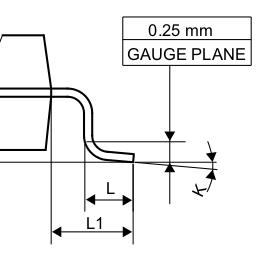
\includegraphics[width=0.7\linewidth]{docs/gullwing_leads.png}
			\caption{OBC MCU Mechanical drawing}
			\label{fig:sub1}
		\end{subfigure}%
		\begin{subfigure}{.5\textwidth}
			\centering
			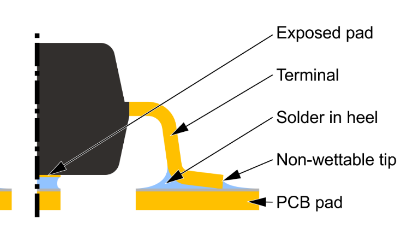
\includegraphics[keepaspectratio, width=1.3\linewidth, height=.4\textheight]{docs/gullwing_solder.png}
			\caption{A perfect soldering of the lead with PCB \small{(\href{https://web.archive.org/web/20200818154144/https://www.infineon.com/dgdl/Infineon-Board+Assembly+Recommendations-Gullwing-Package-v04_00-EN.pdf?fileId=5546d4626d82c047016d8c0320de42d0}{image source}})}
			\label{fig:sub2}
		\end{subfigure}
		\caption{}
		\label{fig:test}
	\end{figure}
	
	%Can you use conductive adhesives for chips based on leadframes or packages with leadframes ? Until now the only reference we have is that solder paste is used mostly in the J leads aka gullwing (\href{https://sst.semiconductor-digest.com/2000/10/lead-free-solders-vs-conductive-adhesives/}{source})
	
	
	%LQFP is a type of package with a leadframe. So the model and the internal structure is the lead-type with wirebonds that have been described previously.
	
	
	
	Now let's examine the dimensions of these gullwing\footnote{The J shaped leads are the so called gullwing leads} leads. The range of values for the depicted L parameter, according to the OBC MCU datasheet, is 0,45 - 0,750 mm and the typical value is 0,6 mm. As we can see from the figures, the exact contact area is a little bit unclear. The solder paste is applied to the whole surface of the PCB pad (this is valid from the .bxl files\footnote{.bxl file extension is a vendor standardized format that can be used via Ultralibrarian software to export data such as schematic symbols, footpritns, 3D models compatible for a wide range of CAD tools.} from ST Microelectronics in which there is metadata for the solder paste layer) and only the L part of the lead is attached to the solder. But all together are electrical and thermal conductive. So we can assume as contact area the PCB pad? In other words the contact area is the L * (width of the lead, that is typically 0.220 mm) or the soldered PCB pad (1.35 * 0.35 mm). It is worth mentioning also that leadframe based packages don't usually touch the surface of the PCB due to the \textbf{standoff} height. The value for this according to the mechanical drawing can range from 0.050 - 0.150.
	
	In order to determine the thickness of the solder paste we need to know the stencil design. A typical value will be 130um.
	
	%All of the above was only for a specific package, the LQFP and the AcubeSAT's PCBs has many different packages. These packages can be divided (or to the leaded and the leadless) to those with leads and the lead-less (dont be confused with the solder paste, the word "lead" is used again, what a coincidence). Actually we need to demystify the terminology of the word packaging. There is the electrical and the IC packaging. The first one is refered to the all kind of interconnections (the die with the leadframe, leadframe with the PCB) and the second one is referred to the encapsulation, the mold-process of the IC. Die, chip, semiconductor are terms used interchangeably. 
	
	\subsubsection{Soldering}
	
	%A word about solder paste. The concern for prisma, solder paste theral properties,conductive adhesive and so on.
	
	For the bonding of two metal surfaces there are two main methods 1) \textbf{electrical conductive adhesive} and 2) \textbf{solder paste} (solder with flux). 
	
	%In the above section we make the assumption that solder is used for the interconnection, but actually this is need to be verified because in the pb-free, green approach other materials may be used except the green solder thing.
	
	Conductive adhesive is a composite of thermosetting epoxy adhesive resin and conductive metal (or metal-coated) particles, such as silver, nickel, gold, copper and indium or tin oxides. On the other hand, the solder is a metal alloy and can be divided to the solder with lead (tin-lead, SnPb) and the lead-free. For the first, the most common is the 63Sn37Pb but due to environmental and health concerns, lead usage is prohibited by regulations (RoHS, REACH) so manufacturers are tending to avoiding it. Tin (Sn) and tin-silver-copper (SnAgCu) belong to the lead-free group. In terms of thermal performance, thermal conductivity is higher in solders (60-65 W/mK) than adhesives (3-25 W/mK) \cite{leadvssolde}. 
	
	The assembly provider of the in-house AcubeSAT's PCBs is Prisma Electronics. It is unclear which of these two methods in the FM models will be used, so clarifications should be requested. Nevertheless if we know the type, then we can retrieve thermal data from these references \cite{solder, wiki:solderalloys, propemetalengedge}.
	
	
	% wave soldering AND adhesive bonding? solder?
	%In the industry there are two main methods to bond the SMDs with the board: 1) adhesive bonding and  wave soldering 2) solder paste and reflow solder. (the last sentences are for SMT and through hole. Both cases an be used solder and conductive adhesive. So refactoring. 
	
	%\href{https://www.electronics-cooling.com/2006/08/thermal-conductivity-of-solders/}{source} for thermal conductivty
	%\href{https://sst.semiconductor-digest.com/2000/10/lead-free-solders-vs-conductive-adhesives/}{source} solder vs adhesive
	%a note about outgassing \href{https://www.masterbond.com/newsrelease/ep21tdcs-lo}{outgassing}
	%\href{https://www.engineersedge.com/properties_of_metals.htm}{table solder alloys all i want}
	%\href{https://www.engineersedge.com/properties_of_metals.htm}{link}
	% this is probably for the assembly of the Eurocircuits
	%The solder paste,the material used to connect the leads of the semiconductors with the pads and the PCB according to \href{https://www.eurocircuits.com/downloads/}{Eurocircuits documents} is the \href{https://www.eurocircuits.com/wp-content/uploads/PDS-SENJU-M705-LFAC19.pdf}{\textbf{M705}}. This document provides the alloy composition but no thermal characteristics.
	
	%. In general terms soldering is preferred with the J-leads like those in the LQFP package. The same applies to the solder paste. Whar solder paste, what type of lead free? 
	
	%\textbf{Comment}: In the thermal simulations that I encountered during this week, solder paste isn't included in the modeling process. Maybe it would be overkill if solder paste is an added node and the complexity will be increased without significant benefits for the uncertainty aspect. But keep in mind this is a comment from a noob in analysis and simulations.
	
	\subsubsection{Closing}
	
	%Check the par before entering the LQFP. Similar notes have been written with the below par
	
	If you have stayed until the end of this package analysis you will realized that the die anatomy and what is inside of the black box is a little bit complex from a thermal's point of view because there is a variety of materials that can be used and many surfaces are touching each other with different physical (thickness, size) and thermal characteristics. For the rest of the packages we will not approach them with the same detail. We will make an overview and if more accurate thermal data is required for the packaging, further research should be made!
	
	
	%Also it should be noted that the above are not either a full detailed analysis of QFP and for the simulation part to this level more information may be required if it is necessary for such an analysis in the PCB/package level. So for that we need to contact with each manufacturer that the materials declaration isn't included in the docs and simulation aspect of the IC is also required due to the increased complexity of the geometries a more heuristic approach should be followed. This approach is unknown and it is not listed. It is just an overview to understand if actually we need to have so much detail in the thermal aspect simulation. That was a flow, it is needed refactoring.!!! 
	
	
	
	\subsection{TSOP}
	
	
	
	Another package, that is included in the group of packages used in the AcubeSAT's boards, is the thin small outline package (TSOP). All the memory modules belong to this category (OBDH MRAM, ADCS SRAM, SU SRAM, SU NAND). This type of package has the leadframe-style and  the mechanical dimensions of the gullwing leads for OBDH, ADCS and SRAM are the same with the previous LQFP and for the SU NAND, the range is 0.4-0.6 with typical 0.5 mm. 
	
	For each one of the memory modules the material declaration is not included in the docs, so we don't know: 1) the terminal plating, 2) base material for the leads. Specifically for OBDH MRAM, from \href{https://www.everspin.com/supportdocs/MR0A16AYS35R?npath=}{a product change notification} about the molding compound used, we can see the code-name "\textbf{Sumitomo G631H}" that is the same in the material declaration of the ST's LQFP packages. So for the Everspin's MRAM we can safely assume that the encapsulation characteristics are the same with the LQFP. For the terminals plating we can assume again that the base material is copper or a copper alloy (or iron\footnote{The material declaration \cite{alliancematdoc} for another TSOP product by Alliance indicates leadframe is iron-based} based) with tin or nickel over gold plating. For clarification, we should contact the vendor.
	
	About the NAND memory module, according to the \href{https://drive.google.com/file/d/1wkUdeeUTbI0Y1cVbS6Vn8aBa2U0LKccN/view?usp=sharing}{user guide}, the leadframe is plated with the usual matte tin or Ni/Pd/Au and the thickness is specified, but it isn't clarified which one of these is used in our particular module. The thickness though is a valuable info (for the standardized world of electronics) and we can use it as a general reference for plating leadframe thickness too.
	\begin{itemize}
		\item Nickel 0.5 um to 1.2 um
		\item Gold 0.003 to 0.012 um
		\item Palladium 0.03 um to 0.11 um
	\end{itemize}
	
	
	
	\begin{figure}[h!]
		\centering
		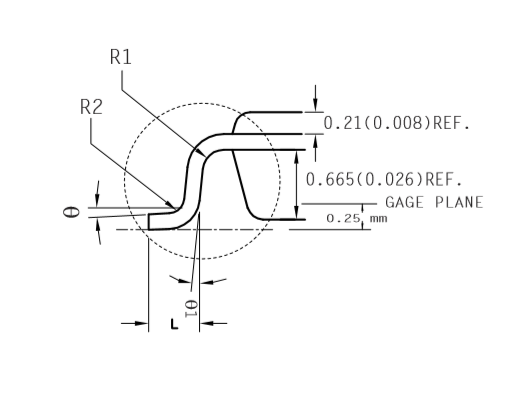
\includegraphics[height=0.3\textheight, width=\textwidth, keepaspectratio]{docs/gullwing_leads_TSOP.png}
		\caption{Gullwing leads for the TSOP2 package by MRAM technical note}
		\label{fig:my_label}
	\end{figure}
	
	\subsection{QFN}
	
	
	Quad Flat No-leads (QFN) package is used for the COMMS AT86RF215 UHF TX-RX. It belongs in the leadless family and includes an exposed thermal pad for heat dissipation (it is recommended to use vias). Usually the package is plastic and the leadframe copper but the material declaration is missing for this specific component. 
	
	It should be emphasized that although there are no leads, according to the datasheet the standoff height range is 0 - 0.05mm (typical 0.02mm).
	
	\begin{figure}[h!]
		\centering
		\begin{subfigure}{.5\textwidth}
			\centering
			\includegraphics[keepaspectratio, width=0.8\linewidth, height=.4\textheight]{docs/qfn_sideview.png}
			\caption{}
			\label{fig:sub1}
		\end{subfigure}%
		\begin{subfigure}{.5\textwidth}
			\centering
			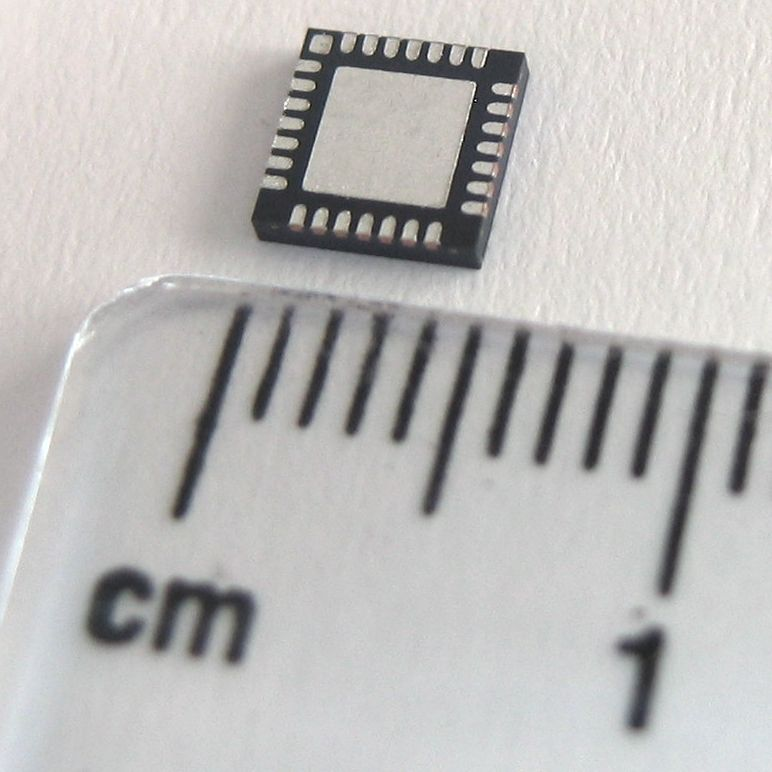
\includegraphics[keepaspectratio, width=0.5\linewidth, height=.3\textheight]{docs/qfn_real.jpg}
			\caption{}
			\label{fig:sub2}
		\end{subfigure}
		\caption{QFN \small{(\href{https://web.archive.org/web/20200818153946/https://en.wikipedia.org/wiki/Flat_no-leads_package}{image source})}}
		\label{fig:test}
	\end{figure}
	
	
	
	%One of the primary goals for the thermal control subsystem is to guarantee the temperature of each chip/junction to stay within specified temperature ranges.
	
	
	
	%what is exactly flux. Demystify the definition and if we need to take into account the flux? Everyone use the same word for solder and solder paste. So what about the flux?
	
	
	\subsection{SOIC}
	
	A Small Outline Integrated Circuit (SOIC) is the package of the EPS TPS54339EDDA. It has 8 pins with an exposed pad. The  \href{https://web.archive.org/web/20200818133800/https://www.ti.com/materialcontent/en/report?pcid=263544&opn=TPS54339EDDA}{material content} is listed in the documentation. It uses a similar leadframe Copper-Iron based with the LQFP, the plating is tin (Sn) and for the encapsulation, a typical epoxy mold compound is used (epoxy resin + fused silica). 
	
	
	
	\subsection{Custom package by Analog}
	
	The ADCS Gyro is consisted of two parts. The ADXRS453BEYZ for the z axis and the ADXRS453BRGZ for the pitch and roll. The first one is a low-cost SOIC package but the second one is different with what we have encountered so far. It is a custom leadless "innovative vertical mount package (VMP)", as Analog Devices states, with ceramic materials. It has two terminals. One in the bottom and one in the back. But as Analog Devices claims only the bottom should be used, the other is for internal evaluation purposes. 
	
	\begin{figure}[h!]
		\centering
		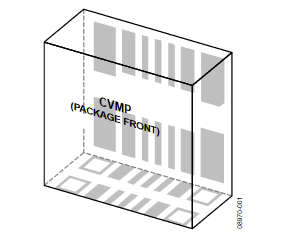
\includegraphics[keepaspectratio, height=.3\textheight, width=\textwidth]{docs/vmp.png}
		\caption{Vertical Mount Package}
		\label{fig:my_label}
	\end{figure}
	
	According to the \href{https://web.archive.org/web/20200818133905/https://www.analog.com/media/en/package-pcb-resources/material-declaration/lcc/LCC_V_14L(ey-14-1).PDF}{material declaration}, the substrate is aluminum-oxide based, a common ceramic solution and the metal lid iron/nickel. The plating is gold/nickel. The ceramic base will have better thermal performance than the rest of the epoxy mold compounds. So for this package a different model approach may be required. But it should be noted that what is referred exactly as lid and base in terms of dimensions is unclear. 
	
	\subsection{LGA}
	
	The Land Grid Array (LGA) is an advanced packing method and this is for the COMMS RFFM6406 UHF TX-RX. It is leadless and it has an exposed thermal pad. Material declaration is missing. We can assume for now that it is plastic based (so we can use LQFP thermal properties as reference), because according to \href{https://web.archive.org/web/20200818134018/https://www.nxp.com/docs/en/application-note/AN2265.pdf}{NXP's application note}, the LGA in the construction is identical with the PBGA except the solder balls. 
	
	About plating: "The LGA pad uses the same 0.1 um to 0.9 um of electroless gold plating over electroless nickel as has been used reliably for many years in the traditional BGA configuration" \cite{nxpplating}.
	
	
	\subsection{Thermal characteristics}
	
	%In order to be able to assess a system designer the thermal performance of an IC package, suppliers usually provide some thermal characteristics that are based on standardized procedures. One of the most used standards for this is the JESD51 series that define the test boards and the conditions of the thermal simulation. 
	%According to TI application note, it is recommended to not use this tool for thermal analysis, but only for comparison if the components are compliant with the same standard.
	%According to the most used standard for this kind is the JESD51. The test boards are this and this. The thermal resistance values so are the indicators of the IC package performance, but ...
	%But how can someone use this thermal data despite having a board different from the test assumption? 
	%In general, each manufacturer may use different standards to evaluate the thermal characteristics. So when trying to find out which package should be used (with a quick assessment), emphasis should be also given to what standards is compliant the test method, what were the conditions of the measurement. If they are the same for the components then probably a reliable assessment can be made. Is this simulation or real, though? 
	
	Until now we have investigated the anatomy and the materials of some IC packages along with its properties. But in the thermal modeling aspect, in order for the supplier to give to the users an overview of the thermal performance, a standardized approach is usually followed. Under the section "Thermal characteristics" or "Thermal metrics"in datasheets,  there is data that can be used to evaluate the junction temperature. This data is produced by thermal simulations with defined by the standards conditions and test boards.
	
	The so called \textbf{theta} values are the indicators of this performance and some of them, using the resistor model, are defined as the thermal resistance between 1) die and ambient, 2) die and case, 3) case and ambient.
	
	\begin{figure}[h!]
		\centering
		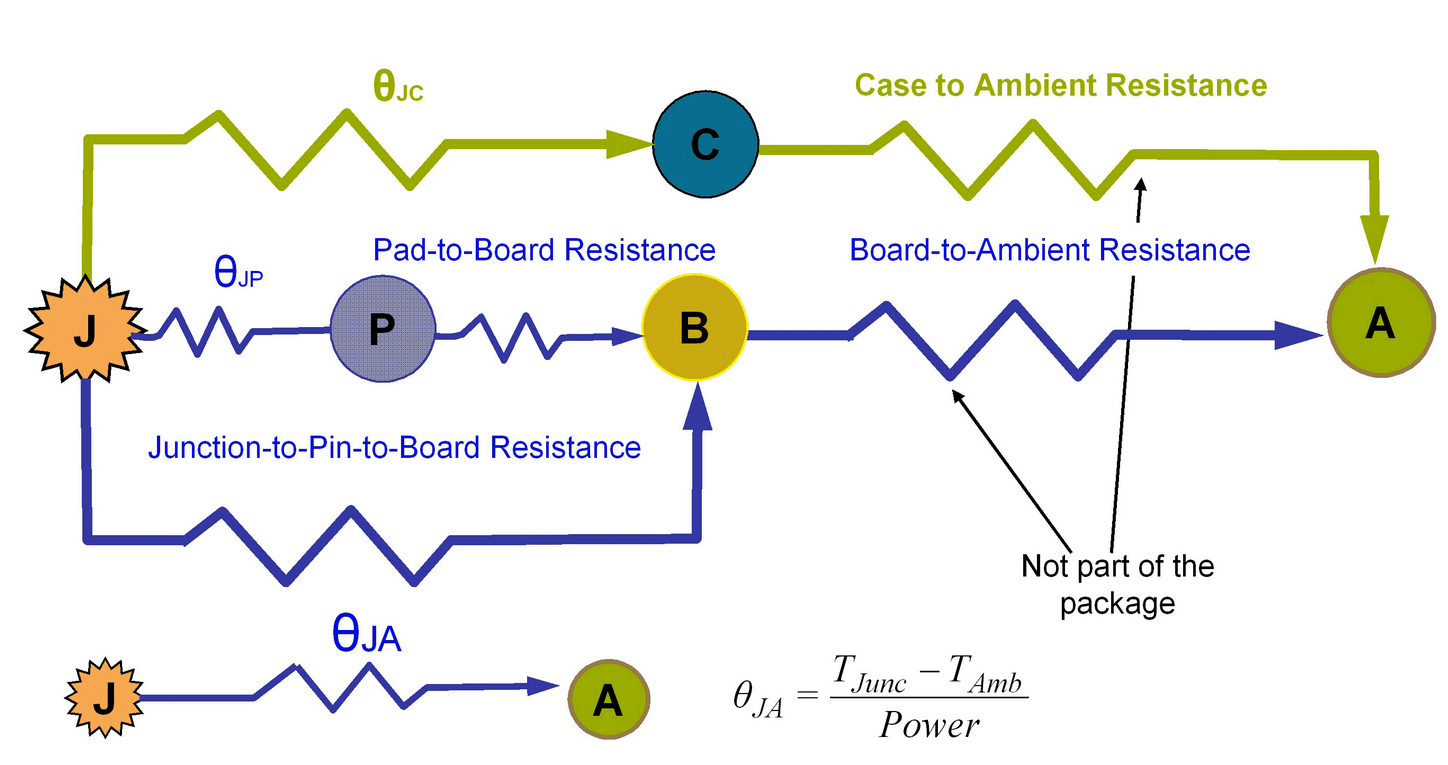
\includegraphics[keepaspectratio, width=\textwidth, height=.25\textheight]{docs/resistor_model.png}
		\caption{A resistor model of an IC package thermal analysis \small{(\href{https://web.archive.org/web/20200818173736/https://www.edn.com/ensuring-the-thermal-integrity-of-your-ic-package-pc-board-design/}{image source})}} 
		\label{fig:my_label}
	\end{figure}
	
	But most of the times, these theta values are not constant and not applicable for every experimental case. According to the \href{https://web.archive.org/web/20200818184640/https://www.st.com/resource/en/application_note/dm00395696-thermal-management-guidelines-for-stm32-applications-stmicroelectronics.pdf}{ST thermal management document}, this data is used for an early assessment and not for a detailed approach. But the questions still remains: Can you use these thermal metrics to your analysis/simulation?
	
	Another usage of this data is to compare the thermal performance of different components. This is only accurate though if all the the values are based on the same standard.
	%In general, each manufacturer may use different standards to evaluate the thermal characteristics and the thermal metrics may be unreliable due to the fact that the conditions that the simulation took place was very specific. In other words the theta values are not constants and they may used for a 
	
	%We will talk about here for the theta values and the abstract thermal model that the vendors are offering as thermal data for the component. The question if I can use this type of values or if this is what I only want for my thermal analysis are very good questions and concerns. In most cases only the theta values aren't enough (reference ee times). But how to read those values, a new introduction to this topic plus application notes and so on and blogs. The first part I will rephrase it until I get in the flow!
	
	%There are thermal characteristics, though. The theta values and so on. But what is the standard approach to characterize the thermal performance of an IC. JEDEC standards and more specific the JES-51 series are the ones that are used a lot in the industry along with the IPC. The JES, open-access, IPC paywalls, closed. But in the thermal characteristics part of the docs of every manufacturer, these values are in compliance with the JEDEC, so we can use them as a reference to demystify how IC providers extract thermal data.
	
	\subsubsection{External links}
	\begin{itemize}
		\item \href{https://web.archive.org/web/20200818132243/https://www.ti.com/lit/an/spra953c/spra953c.pdf}{TI Semiconductor and IC Package Thermal Metrics}
		\item \href{https://web.archive.org/web/20200818123847/https://www.nxp.com/docs/en/white-paper/BasicThermalWP.pdf}{NXP Thermal analysis of semiconductor devices}
	\end{itemize}
	
	
	\section{PCB}
	
	In the "Buildup" section, when ordering from Eurocircuits, there are many options for the thickness of the core FR4 and the copper foils.
	
	Approximate thickness values for a typical 4 layer board 1.55\footnote{In the board thickness only the copper and the dielectric is taken into account} mm:
	\begin{itemize}
		\item FR4:  1,4 mm
		\item Copper:  0,15 mm
		\item Soldermask: 35 - 40 microns
		\item Surface treatment: 20 - 25 microns
		\item Conformal coating: -
	\end{itemize}
	
	
	\begin{figure}[h!]
		\centering
		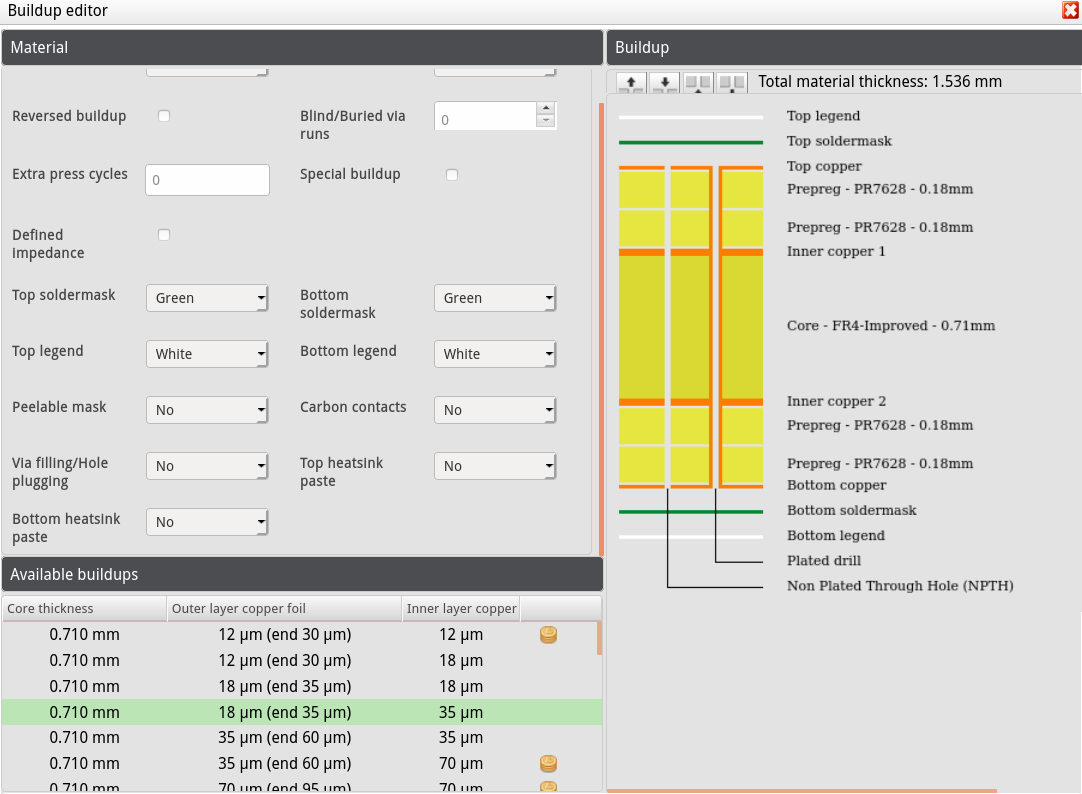
\includegraphics[keepaspectratio, height=0.35\textheight, width=\textwidth]{docs/stackup.png}
		\caption{A typical 4-layer board ordered from Eurocircuits}
		\label{fig:my_label}
	\end{figure}{}
	
	
	\subsection{FR4}
	
	\textbf{IS400}, for example, is one of the  available options by Eurocircuits for FR4 substrate. In general FR4 in contrast with others more expensive ceramic substrates based on aluminum and silicon has a low thermal conductivity. So if there are thermal issues, FR4 replacement is also a choice. Usually ceramic substrate thermal conductivity (typically 10 W/mK) can be 10 or even 100 times greater than FR4 (typically 0,3 W/mK) \cite{zotero-57, zotero-56}. For the IS400 we have:
	
	\subsubsection{Documentation}
	
	\begin{itemize}
		\item \href{https://www.isola-group.com/products/all-printed-circuit-materials/is400/}{All files}
		\item \href{https://web.archive.org/web/20200818140037/https://www.isola-group.com/wp-content/uploads/IS400MaterialDeclaration2007.pdf}{Material declaration}
		\item \href{https://web.archive.org/web/20200818140113/https://www.isola-group.com/wp-content/uploads/data-sheets/is400.pdf?v=1585950502}{Datasheet}
	\end{itemize}
	
	
	\subsubsection{Thermal properties}
	
	\begin{center}
		\tablehead{\hline}
		\tabletail{\hline}
		%\tablecaption{FR4 samples of thermal properties}
		\begin{mpsupertabular}{|c|c|c|}
			\multirow{1} {*} {Thermal conductivity (W/mK)\footnote{Reference for the thermo-optical properties \href{https://web.archive.org/web/20200818140113/https://www.isola-group.com/wp-content/uploads/data-sheets/is400.pdf?v=1585950502}{datasheet}}} & 0,36 \\  
			\hline
			\multirow{1} {*} {Heat capacity (J/kg*K) \footnote{References for the thermo-optical properties Figure \ref{fig:fr4properties}}} & 1000 \\ 
			\hline
			\multirow{1} {*} {Emissivity  \footnote{References for the thermo-optical properties Figure \ref{fig:fr4emiss}}} & 0,9  \\
			\hline
			\multirow{1} {*}{Absorptivity  \footnote{References for the thermo-optical properties Figure \ref{fig:fr4emiss}}} & 0,49 \\
			\hline
		\end{mpsupertabular}
	\end{center}
	
	
	
	
	\textbf{Issue}: The thermal properties emissivity, absorptivity and heat capacity are missing from the datasheet. Alternatively, estimations can be made from other abstract resources (e.g. makeitfrom, wikipedia, handbooks, other applications notes from manufacturers, engineering toolbox).
	\newline
	
	%\textbf{Done}: Ask the FR4 supplier to provide the missing thermal characteristics (e.g. emissivity, heat capacity, absorptivity). Hope they will respond (update: they didn't!). If they don't respond, maybe the email format or the approach should be more convincing.
	
	\subsection{Copper}
	
	Detailed data about the Eurocircuit's copper foil is missing from their documents. The only information available is the thickness and the overall process of the fabrication. So we could probably assume that the thermal properties will be the same with the well-known pure copper.
	
	
	\begin{center}
		%\tablehead{\hline}
		%\tabletail{\hline}
		\tablecaption{Copper samples of thermal properties}
		\begin{tabular}{|c|c|}
			\hline
			\multirow{2} {*} {Thermal conductivity (W/mK)} & 401 \cite{wiki:copper} \\ & 20 \cite{chandrashekar2017} \\ & 392 \cite{pecht1998electronic} \\
			\hline
			\multirow{1} {*} {Heat capacity (J/kgK)} & 0,385 \cite{wiki:tableheat}\\
			\hline
			\multirow{2} {*} {Emissivity}  & 0,87 oxidized \cite{wiki:emissivity}\\ & 0,8 \cite{chandrashekar2017}\\ & 0,8 coil tape \cite{nasa} \\ & 0,55 foil tape, tarnished \cite{boushon2018} \\ & 0,31 beryllium \cite{boushon2018}\\  & 0,04 polished \cite{wiki:emissivity}\\  & 0,03 electroplated \cite{chandrashekar2017}\\ & 0,3 buffed \cite{boushon2018}\\ 
			\hline
			\multirow{2} {*}{Absorptivity} & 0,04 foil tape, tarnished \cite{boushon2018}\\ & 0,03 buffed \cite{boushon2018} \\ & 0,31 beryllium \cite{boushon2018} \\ 
			\hline
		\end{tabular}
	\end{center}
	
	%\textbf{Notes}:
	
	%\begin{itemize}
	%    \item Beryllium reference is for other usages like solar absorvers or antenna design in the spectrum of spacecraft thermal engineering. In some cases copper beryllium is used as a base metal for connectors too (the pins)
	%    \item Satellite thermal control handbook has great refernces about the validity of the modeling. USed also as a base metal for connectors, pins
	%    \item Should be noted that these values of pure copper may not be used, following a different approach and use experimental data of PCB structure as an homogenous material. A lot of references about this 
	%\end{itemize}
	
	%\subsection{Coatings}
	
	%About conformal coating I will be redirect you to the section of this book the electronics packaging handbook and so on.
	
	%In the PCB fabrication there are many steps invovlved in the fabrication cycle and there are many terms about the "coating" but they are different. These are:
	
	%\begin{itemize}
	%    \item Conformal coating
	%    \item Adhesives
	%    \item Soldermask
	%    \item Surface treatment
	%    \item Peelable mask. It is involved only in the fabrication and later is removed. So it %  %    doesn't affect the user, so don't care.
	%    \item other
	%\end{itemize}{}
	
	% Conformal coating (first time exposed to this term by  \cite{mccarron2018developing}) is an additional type of coating that is part of the assembly process. It is used for additional protection and to improve overall performance (I have more notes about this)and for that and that, these types. \textbf{It should be noted that if conformal coating wll be part of the design and what type should be, it is something that until now hasn't been investigated yet}. But the presence of it as this paper claims, will affect the thermal radiation aspect of modeling. The same is unknown for additional thermal adhesive.
	\section{PC104}
	
	I am going artfully redirect you to the following reference:
	
	"Concerning the conductive links between the PCBs, there are two main heat flow paths: through the spacers and through the connector. According to the PC/104 specification, the connector is made up of 104 phosphor bronze pins and only pins contributes to the link since connector’s housing height is such as there is no contact with the above PCB". Thermal conductivity of Phosphor bronze 75 W/mK \cite[p.104]{jacques2009thermal}. 
	
	
	
	\section{Lessons learned}\label{lessons_learned}
	
	In the beginning of the research, the thinking path about finding materials was oriented to search for each manufacturer the "material declaration" document. Knowing the materials, we will be able to find its thermal properties. But for each part of the component we are interested (e.g. encapsulation) a mixture of materials is used. Thus we assume that we need to focus on the material with the highest concentration. Later for optimization we could find the thermal properties of all them along with a formula to calculate the overall performance. This approach may be not be valid and probably should be avoided. The primary reason is that this concept is error-prone and adds significant load, trying to demystify the thermal properties of each material and for each component, lacking at the same time the resources to find reliable data. A more abstract way of thinking is may required. So as it is mentioned before, in the IC packaging, a process which several chemical compounds are involved, we can safely assume the general model of an epoxy mold compound for the plastic packages. The same homogenous approach applies for the FR4 too, but fortunately we were able to find experimental data for our case provided by the supplier.
	
	%Give an example of conductive adhesive that is polymer with metal. Assume that only polymer then all the thermal characteristics of the metallization will be lost in the void. It is very important to treat it as composite material.
	
	When approaching the material properties of a mixture of materials, there are many chances that what you are looking for has some kind of a code-name, a specific composition. These are common alloys and it would be helpful to identify it by checking the composition from the material doc. 
	
	%Should I say here also the thing with what? The matrix of materials, with nodes if you know the thickness and the process example with pins anf bronze, I have a reference in the pcb modelling for that!
	
	\subsection{Modeling}
	\label{subsec:modeling}
	
	%latex is weird. Previously the \subsection didnt work, but now okay
	
	
	%Theere are  many ways that the PCB can be modelled. First of all it is needed to be determined if it will be approached as an homogenous material or as a sandwich of copper and dielectric layers. But for the second method how many layers and what about the geometry of tracks and the vertical interconnection path (via) that can maybe result in a much different thermal analysis. We should not forget that thermal pads along with vias that connect the top layer with the bottom layer can probably change significantly the heat dissipation of a thermal crucial component. Some references of PCB modeling approaches will be listed:
	
	%For the homogenous approach the PCB assumed as an epoxy, fr4, copper body. The formula that is used and so on, put citation
	
	In some case we find modeling the PCB as an homogenous material and it is worth mentioning them:
	
	%We find some references regarding the PCB modeling and it is worth mentioning them:
	
	"Printed circuit boards (PCBs) are complex structures usually made up of layers of copper and glass fiber reinforced (fiberglass) epoxy resin, making them difficult to model directly. The layered structure and sharp difference in thermal conductivity between materials leads to highly anisotropic thermal conductivities. Since actually modeling each layer at such small scales and in such detail requires a lot of computational effort and time, the typical practice is to treat the circuit board as a homogenous material and use an effective thermal conductivity" \cite{peake2014cubesat}
	
	\begin{figure}[h!]
		\centering
		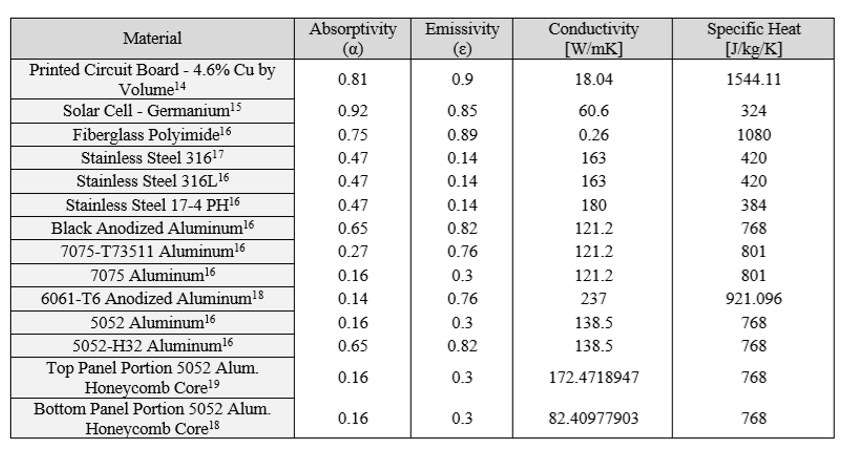
\includegraphics[keepaspectratio, height=0.3\textheight, width=\textwidth]{docs/material_properties_table.png}
		\caption{Material properties table  \cite[p.115]{zotero-47}}
		\label{fig:my_label}
	\end{figure}
	
	A list of concerns:
	
	\begin{itemize}
		\item "An especially intriguing problem shows up when printed circuit boards are part of the analysis. The values for the thermal conductivities of PCB’s cited in literature are mostly conductivities of the epoxy in the direction normal to the PCB. However, these values are useless in practice because: a) the thermal conductivity of the reinforced epoxy can be highly anisotropic, b) the in-plane thermal conductivity is much more important from a practical point of view, c) the very complex patterns of metal tracks and layers will considerably influence the thermal conduction behavior" \cite{lasance2002}
		\item ”Regarding the material properties it was found that small changes, e.g.  adding a layer of copper to the circuit board, can significantly decrease the resulting temperatures.  This is due to the improved in-plane conductivity, as copper has an unequally higher conductivity than FR4(Cu=394W/mK compared to FR4=0.3W/mK).” \cite{reiss2012} 
		\item "While the temperature changes significantly, the overall pattern of the heat distribution remains relatively unchanged. The largest change is the difference between the highest and lowest temperatures, which grows from 6 K to 52 K between $\epsilon$ = 0.02 and $\epsilon$ = 0.82. Overall, it is clear that emissivity plays a very significant role in the spacecraft temperature. This was expected, since radiation as a mode of heat transfer is far more important in the near vacuum of space, and is the only mode by which heat can be transferred away from the satellite." \cite{peake2014cubesat}
		\item "Because a satellite in orbit is surrounded by the vacuum of space, its only
		thermal interaction with its environment is through radiation" \cite{vanoutryve2008}.
		
		"The aluminum external surface is the only \textbf{external} part which can be used to control the temperature by modifying the optical properties of the material (with an adequate surface treatment); indeed, the optical properties of the solar cells and of the PCB that are mounted to them cannot be modified" \cite{paris2015}.
		
		Also in the TIGRIsat's simulations , when they didn't take into account the surface treatment of the aluminum structure/rails, the temperature had exceed the maximum one. The reason behind this was the big difference between aluminum's absorptivity (0,379) and emissivity (0,08) due to the aforementioned assumption that there wasn't any surface treatment \cite{paris2015}. Based on that, the input data of "critical" components should be investigated thoroughly and the change of thermal-optical properties can be also part of the strategy.
	\end{itemize}
	
	
	
	%But the term composite and mixture of materials are different. If the composite materials can be define individually as nodes. "Even  mixed  materials  can  be  modelled  in  away that the nodal properties are put together with the  same  ratio  of  materials  being  involved. A connector consisting of copper contacts housed by a plastic casing could therefore be modelled with a mixture of both materials, each contributing its properties in the respective parts" \cite{reiss2012new}
	
	%"Regarding parts with mixed materials these properties  were  approximated  using  the  ratio  of  each material involved.  For the thermal conductivity of the printed circuit boards, the directivity was considered" \cite{reiss2012new}
	
	
	
	%All the fuss for emissivty is for the structure, the frame aluminum alloys and such (something relevant mention has the UPS satelitte). So the emissivity in certain surfaces like the frame should be considered thoroughly.
	
	
	
	
	%About external surfaces and emissivity and so on. Sweep article in the other notes. lets combine the knwoledge.Aluminum surface emissivity. Results of a parameter sweep emissivity in a thermal analysis of such and such
	
	
	
	%"Finally, the emissivity/absorptivity ratio is the main parameter which we can play in order to change these temperature variations" \cite{zotero-52}
	
	
	%If we know the material declaration and all the thermal properties of each substance, how can we approach it to find the thermal properties as an homogenous material. Is it uncertainty-enough/valid to use only the thermal properties of the most concentration's substance?
	
	%"There is a built-in database of commonly used materials and their thermal and optical properties" \cite{vanoutryve2008}. How to find thermal optical properties. According to the paper a thermal design and analysis tool for small satellites. Question derived, esatan has a built in database?
	
	%\textbf{Note}: Material's thermal properties can change quite a lot despite the amount of mass used of other materials. Examples of copper oxidized, electroplated, polished and should find more to prove my point that it is not the concentration is the overall performance. A lot of research have been conducted for thermal enhancements..
	
	%\textbf{About IC packaging. Need refactor}
	%\begin{itemize}
	%    \item In case we don't have the material declaration, we won't know the exact chemical composition of the IC, so we don't know the terminal plating, the base metal. But even if we know them, how can you approach it as an homogenous material. I mean basically the leadframe is a metal or metal alloy. The plating is also a solderable metal alloy. We can find easily thermal properties for each one of those, but how can you define the thermal characteristis as an homogenous lead with base metal and plated too. For the PCB we have the same problem. We know the coppper and the plated. So, one problem is the fact that you don't know the material declaration and the second one after you know the composition and after you find the thermal characteristics (what about the theta values), how homogenous formula?
	%\end{itemize}
	
	\subsection{Uncertainty and thermal properties}
	
	%Thermal properties are indeed a very significant factor to determine a successful prediction  but .... sometimes finding valid ones for each specialized application is a hard thing to do (inaccurate measurement techniques, uncertainty, complexity, a lot of dependencies). The terms "assume" and "estimate" are used very often in the literature. A list of references for proof of concept:
	
	%version 2
	
	Many thermal properties can be indexed. This is true. But most of the times, conflicts will emerge. There is a variety of values referred to the same material and input thermal data is also a part of the engineering process. Assumptions and estimations are  common and they are function of the general modeling approach. Do I need this property, can I model it with another way, how uncertain is this thermal data, is this material oxidized or even if it isn't can I benefit assuming that it is? 
	
	\begin{itemize}
		\item "... models of the electrical and electronic components has been created, despite the \textbf{difficulty} of determining their thermal and optical properties." 
		
		"Indeed, the \textbf{actual} structure of TIGRIsat is anodized but the actual value of $\alpha$  and $\epsilon$ are \textbf{unknown}" \cite{paris2015}
		\item "Often information for properties of individual material is \textbf{unavailable} and, where possible, in-house testing using an emissometer should be performed to acquire it." \cite{mccarron2018developing}
		
		%In the literature about the calculations the words "assume", "estimation" are used quite often!
		
		\item "However, there may be quite a few uncertain or inaccurate input parameters existing in the thermal mathematical model (TTM), which may affect the analysis accuracy, including thermal contact resistance between contacting parts, unit thermal properties (such as thermal capacitance, thermal conductivity, infrared emissivity, and solar absorptivity), unit power dissipation, etc. Therefore, a thermal balance test is essential to verify the basic thermal design and to assure that the TMM is reliable for the temperature prediction because the input parameters are proved to be valid" \cite{tsai2004overview}
		
		%\item The effect of realistic changes in the input values on the resultant temperatures was observed in order to give confidence in the results obtained \cite{butcher1999}
		
		
		\item About the accuracy of experimental and numerical thermal analysis of electronic systems: "The final conclusion is inevitable: the situation when all computations at the system level can be used for accurate temperature prediction is still a long way off" \cite{lasance2002}
	\end{itemize}
	
	With all of that being said we can understand that we can't trust the thermal data. Experimental data for each application along with tests is a necessary part of the design-cycle. In prototypes, thermocouples and infrared cameras can be used in the same way that oscilloscopes are being used for the electrical domain.
	
	\section{Databases}\label{Databases}
	
	%A list of resources for indexing thermal properties:
	\begin{itemize}
		\item Glenn R Blackwell.The electronic packaging handbook.  CRC Press, 2017
		\item Safa Kasap and Peter Capper.Springer handbook of electronic and photonic materials.Springer, 2017
		\item Rao R Tummala et al.  Fundamentals of microsystems packaging.  2001
		\item R.P.  Chhabra.CRC Handbook of Thermal Engineering.   Mechanical  and  AerospaceEngineering Series. CRC Press
		\item  M. Pecht, R. Agarwal, F.P. McCluskey, T.J. Dishongh, S. Javadpour, and R. Mahajan.Electronic Packaging Materials and Their Properties.  Electronic Packaging. Taylor Francis
		\item D.G. Gilmore and M. Donabedian.Spacecraft Thermal Control Handbook: FundamentalTechnologies.  Spacecraft Thermal Control Handbook. Aerospace Press
		\item https://theengineeringmindset.com/specific-heat-capacity-of-materials/
		\item \href{https://www.makeitfrom.com/}{makeitfrom.com}. A general online database for various materials. Mined from Wikipedia references
		\item \href{https://www.engineeringtoolbox.com/}{The Engineering Toolbox}. This reference is used quite a lot.
		\item \href{https://web.archive.org/web/20200818140417/https://monarchserver.com/Files/pdf/TableofEmissivity.pdf?14860239451575071105}{Table of Total Emissivity}
		\item \href{https://web.archive.org/web/20200818140448/http://www.solarmirror.com/fom/fom-serve/cache/43.html}{Table of absorptivity and emissivity of common materials and coatings}
		\item \href{https://drive.google.com/file/d/1nZOXnBw6FdrzXW1Nm0Q7n0jfy6kBI26J/view?usp=sharing}{Thermal Properties of Plastic Materials}
		\item \href{https://web.archive.org/web/20200818140510/http://www.infrared-thermography.com/material.htm}{Emissivity Values for Common Materials}
		\item \href{https://cindasdata.com/Applications/MPMDDEMO}{CINDAS LLC}. This is an interesting database. There are thermal properties even for very specific mold compounds types like "Sumitomo EME-6300HS" (just to remind you, ST is using Sumitomo type mold compounds as encapsulation) but it is proprietary.
	\end{itemize}
	
	
	%\section{Conclusion}
	
	%Why it is hard to find thremal properties, find refernces. I have two in mind. The bible for developing standards space, and the one about fr4 posted in mattermost and one more about the paper with the accuracy and the uncertainty of values. So experimental data for our application should be probably also a very important part of our design. What about facilities. How to prototypes? Services for these kind of measurement to validate our data, but for which conditions? 
	
	%Tests and experimental data are key parts of the design cycle for validation and confidence. These kind of results give valuable feedback to adjust/re-calibrate the models and more accurate predictions will follow up. 
	
	%and more (I can't remember the word for confidence, achieving?) confident, better models, better simulations, better predictions. Feedback loop, better models, accurate data, prediction and so on. But how many stuff we have to validate with our tests? The numerical approach, the modeling, the values. How can you spot which of those you need to calibrate for a better analysis?
	
	
	\section{List of tables}\label{list_tables}
	
	
	
	\begin{figure}[h!]
		\centering
		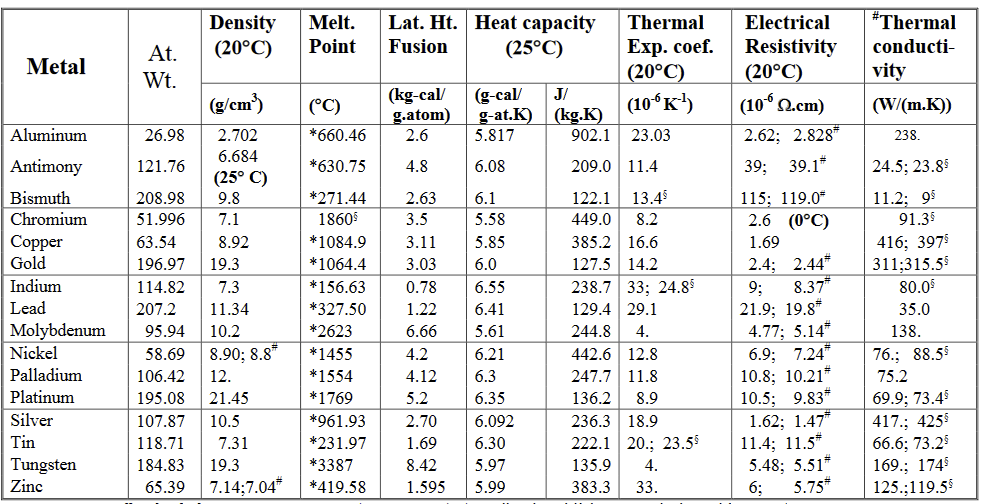
\includegraphics[width=\linewidth]{docs/mist_heat_capacity.png}
		\caption{\cite[p.37]{solder}}
		\label{fig:metal_table_1}
	\end{figure}
	
	\begin{figure}[h!]
		\centering
		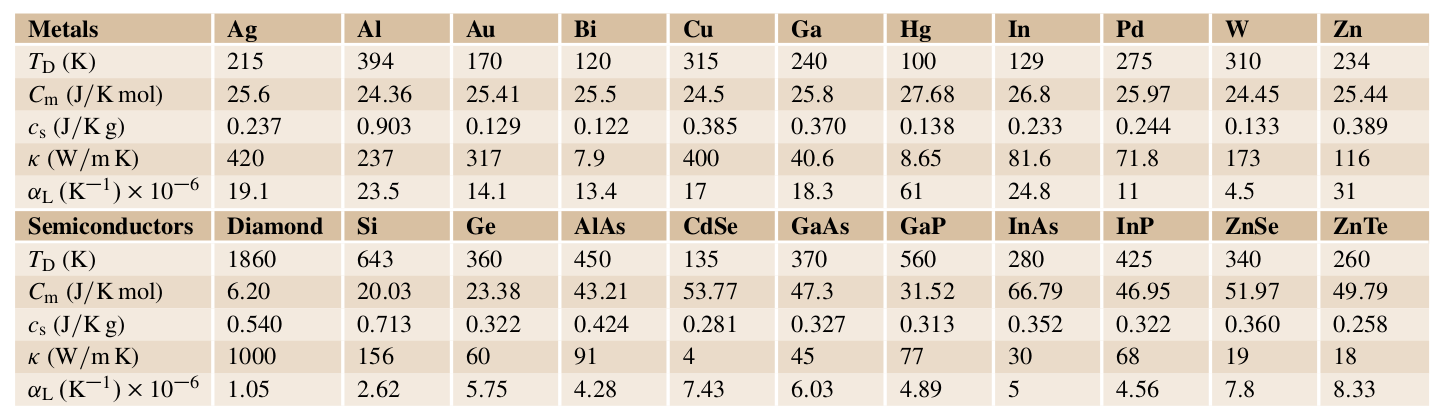
\includegraphics[width=\linewidth]{docs/table_properties_springer.png}
		\caption{\cite[p.428]{kasap2017springer}}
		\label{fig:metal_table_2}
	\end{figure}
	
	\begin{figure}[h!]
		\centering
		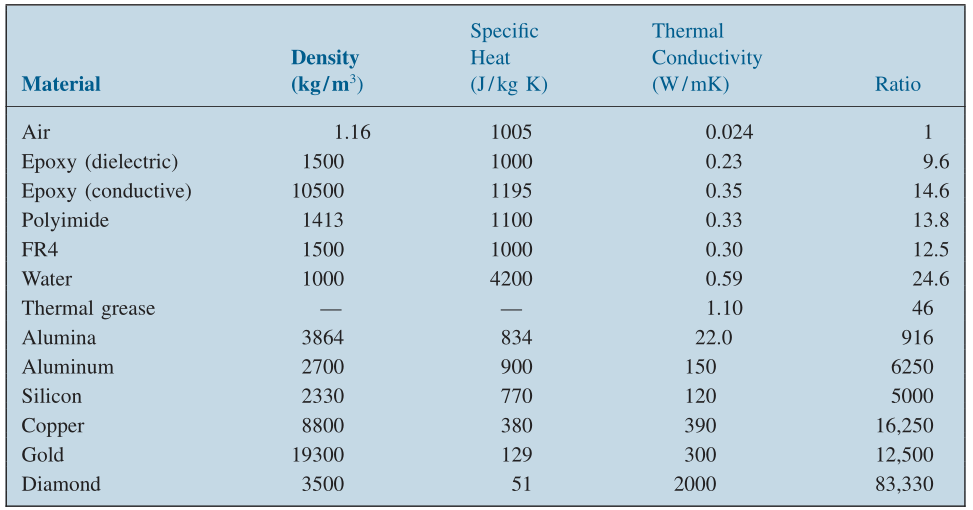
\includegraphics[width=\linewidth]{docs/table_properties_bible.png}
		\caption{\cite[p.222]{tummala2001fundamentals}}
		\label{fig:fr4properties}
	\end{figure}
	
	\begin{figure}[h!]
		\centering
		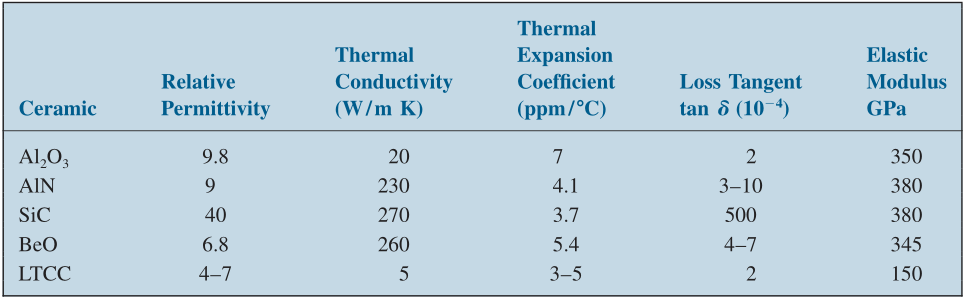
\includegraphics[width=\linewidth]{docs/table_ceramics_bible.png}
		\caption{\cite[p.718]{tummala2001fundamentals}}
		\label{fig:my_label}
	\end{figure}
	
	
	
	\begin{figure}[h!]
		\centering
		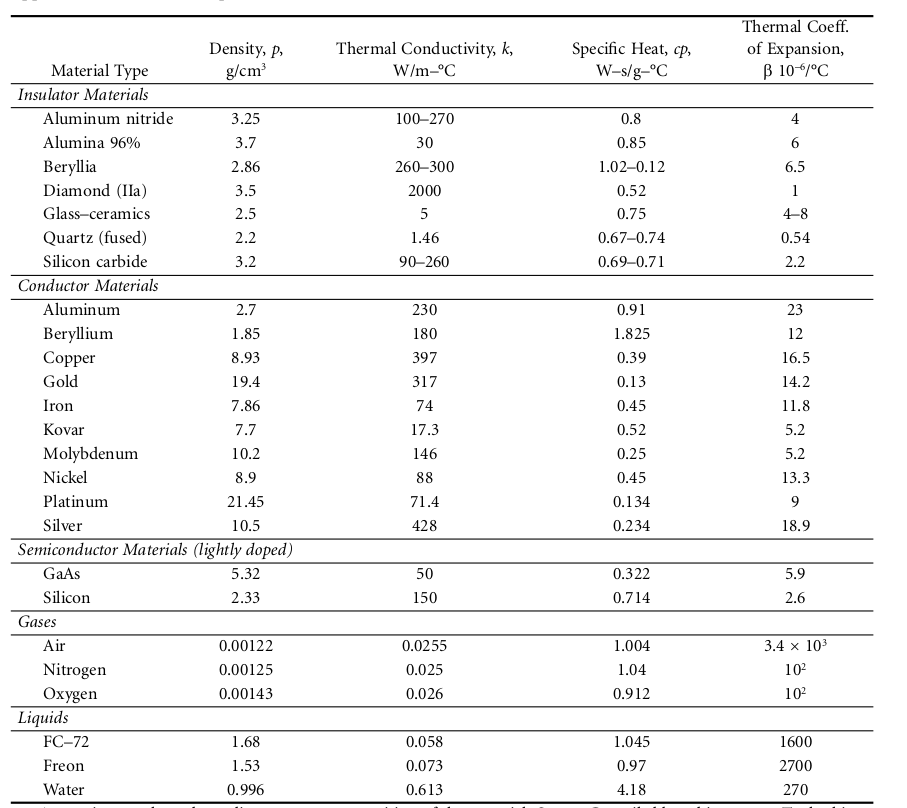
\includegraphics[width=\linewidth]{docs/table_properties_blackwell_handbook.png}
		\caption{\cite[p.408]{blackwell2017electronic}}
		\label{fig:springer_properties}
	\end{figure}
	
	\begin{figure}[h!]
		\centering
		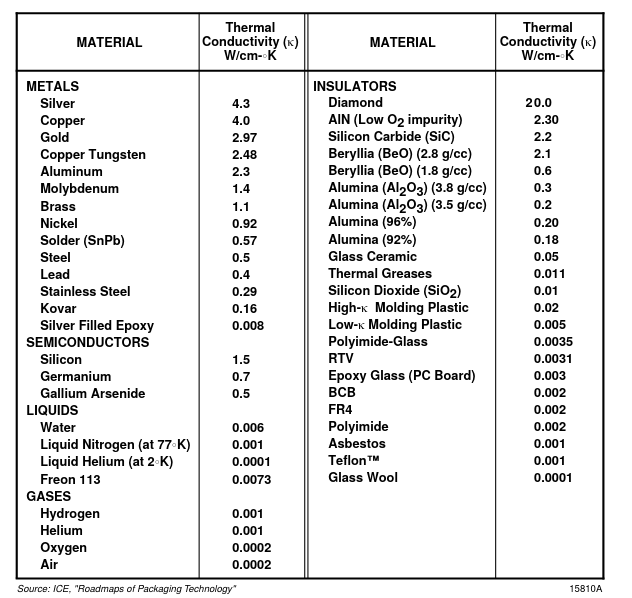
\includegraphics[width=\linewidth]{docs/table_properties_smith.png}
		\caption{\cite[6-14]{chip}}
		\label{fig:intel_conduct}
	\end{figure}
	
	\begin{figure}[h!]
		\centering
		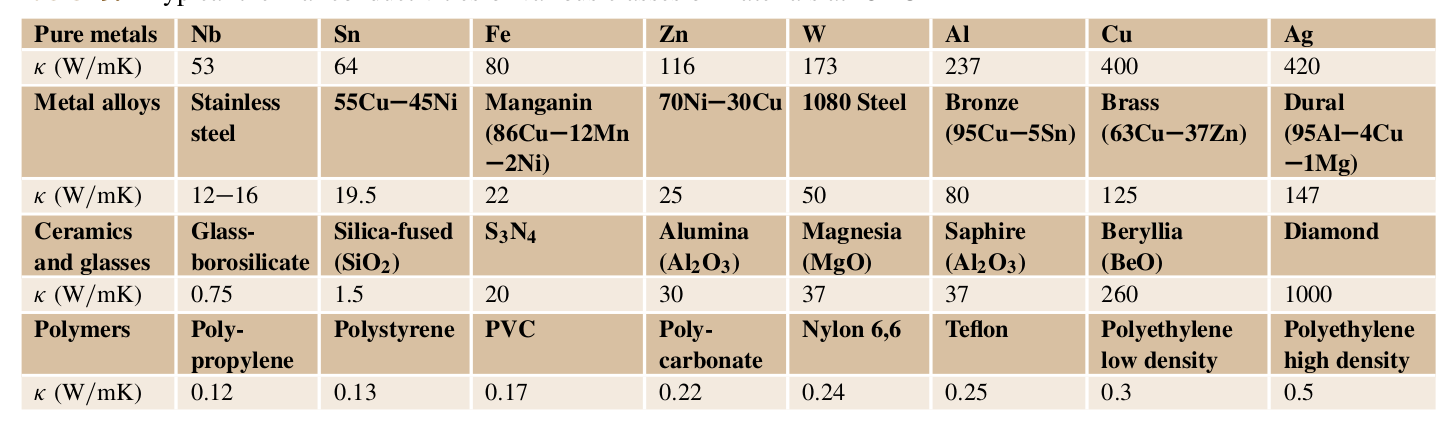
\includegraphics[width=\linewidth]{docs/table_properties_springer2.png}
		\caption{\cite[p.431]{kasap2017springer}}
		\label{fig:my_label}
	\end{figure}
	
	\begin{figure}[h!]
		\centering
		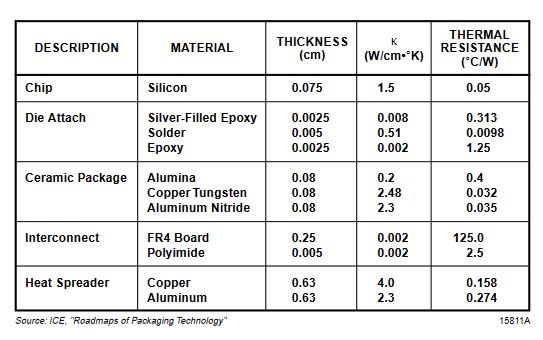
\includegraphics{docs/chip_properties.png}
		\caption{\cite[p.6-12]{chip}}
		\label{fig:my_label}
	\end{figure}
	
	\begin{figure}[h!]
		\centering
		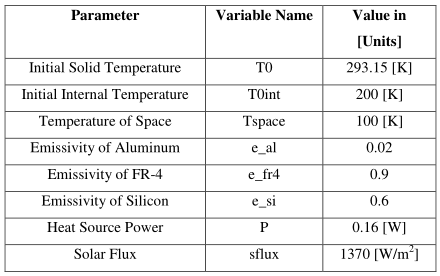
\includegraphics[keepaspectratio, width=\textwidth]{docs/emissivity_silicon_fr4.png}
		\caption{\cite[p.41]{peake2014cubesat}}
		\label{fig:my_label}
	\end{figure}
	
	
	\begin{figure}[h!]
		\centering
		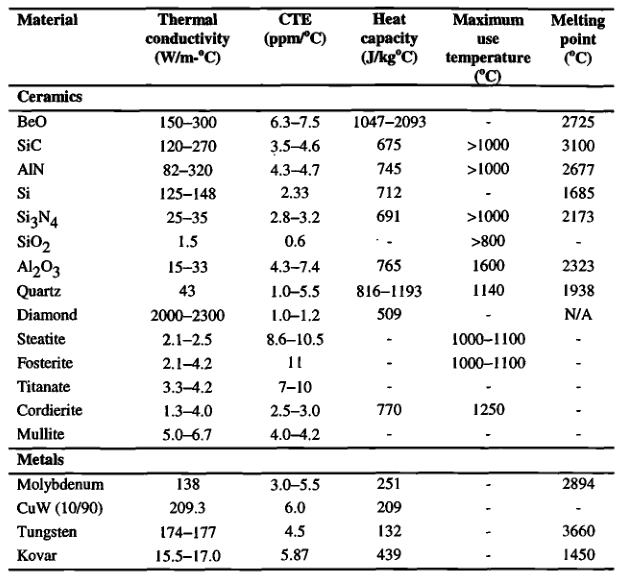
\includegraphics[keepaspectratio, width=\textwidth]{docs/substrates.png}
		\caption{Substrates \cite[p.32]{pecht1998electronic}}
		\label{fig:my_label}
	\end{figure}
	
	\begin{figure}[h!]
		\centering
		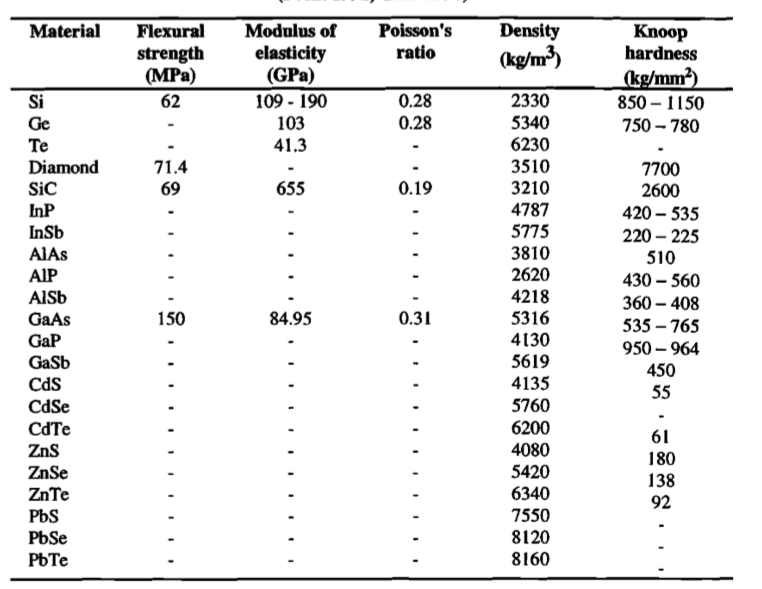
\includegraphics[keepaspectratio, width=\textwidth]{docs/density_table.png}
		\caption{\cite[p.24]{pecht1998electronic}}
		\label{fig:my_label}
	\end{figure}
	
	\begin{figure}[h!]
		\centering
		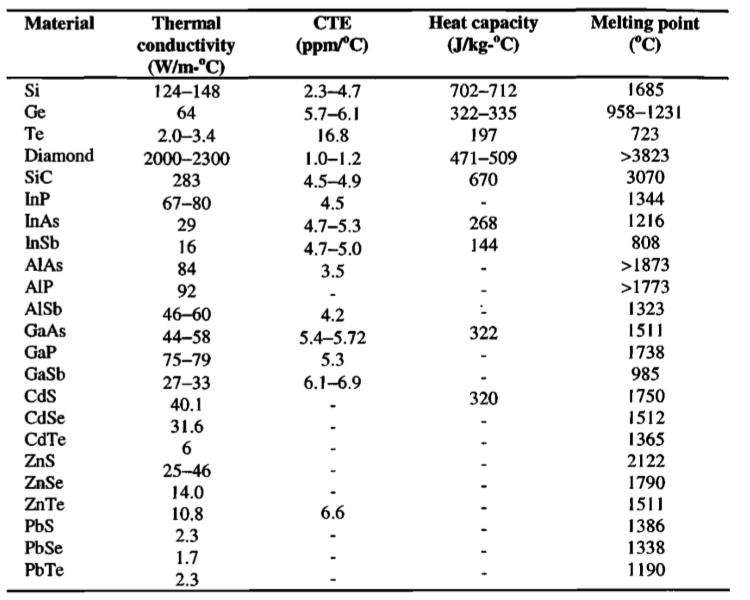
\includegraphics[keepaspectratio, width=\textwidth]{docs/material_overall_properties.png}
		\caption{\cite[p.25]{pecht1998electronic}}
		\label{fig:my_label}
	\end{figure}
	
	\begin{figure}[h!]
		\centering
		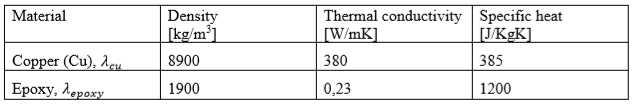
\includegraphics{THE/AcubeSAT-THE-BH-032/docs/homo_pcb.png}
		\caption{\cite[p.20]{airborne}}
		\label{fig:my_label}
	\end{figure}
	
	
	\begin{figure}[h!]
		\centering
		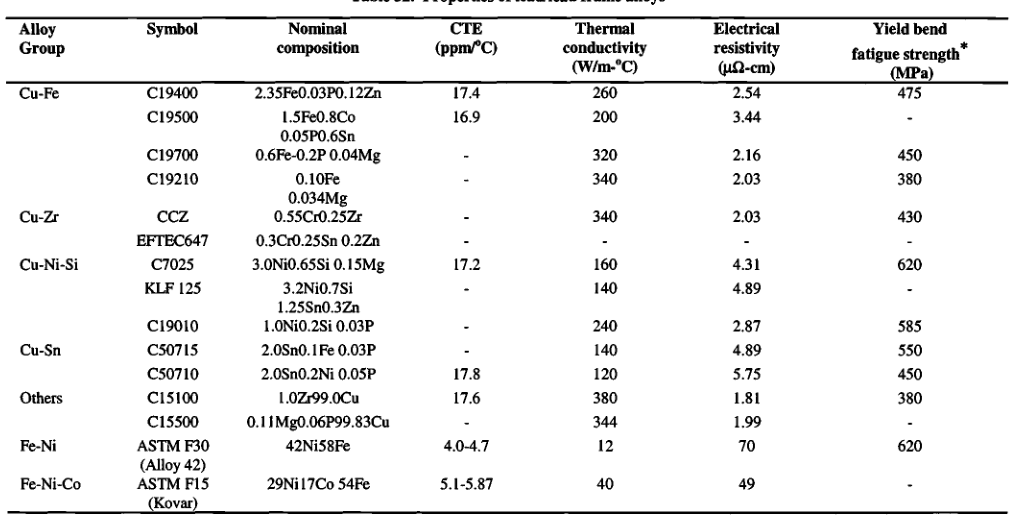
\includegraphics[keepaspectratio, width=\textwidth]{docs/copper_alloys_blackwell.png}
		\caption{\cite[p.55]{pecht1998electronic}}
		\label{fig:copper_alloys}
	\end{figure}
	
	\begin{figure}[h!]
		\centering
		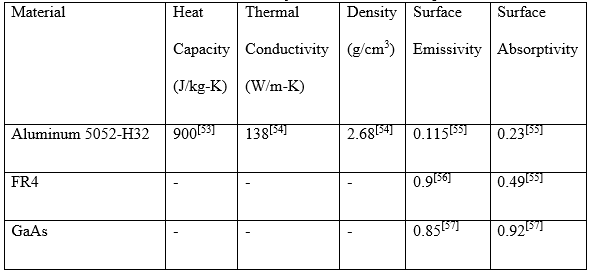
\includegraphics[keepaspectratio, width=\textwidth]{docs/fr4_emiss.png}
		\caption{\cite[p.93]{rathbun2017design}}
		\label{fig:fr4}
	\end{figure}
	
	\begin{figure}[h!]
		\centering
		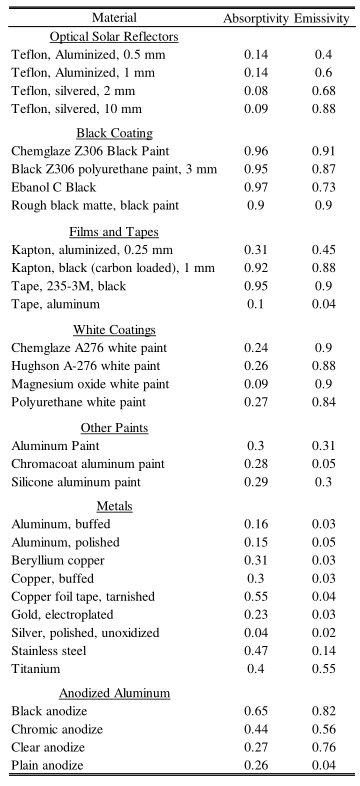
\includegraphics[keepaspectratio, height=.8\textheight, width=\textwidth]{docs/small_sat_properties.png}
		\caption{\cite[p.111]{boushon2018}}
		\label{fig:fr4emiss}
	\end{figure}
	
	\begin{figure}[h!]
		\centering
		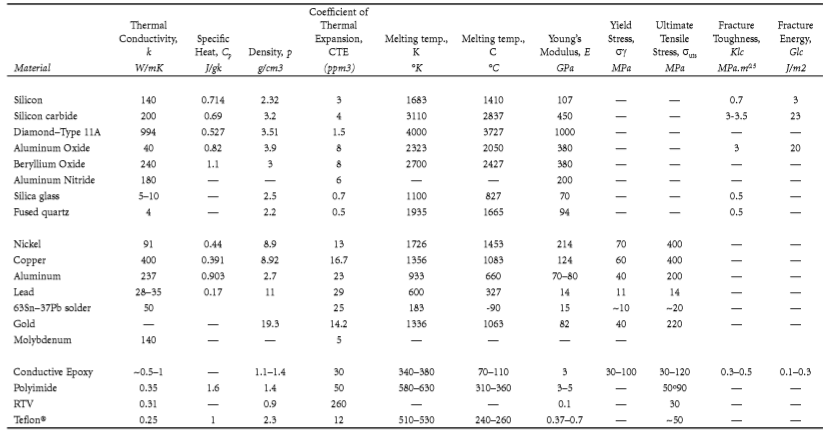
\includegraphics[keepaspectratio, height=.8\textheight, width=\textwidth]{docs/blackwell_prope.png}
		\caption{Metals \cite[p.526]{blackwell2017electronic}}
		\label{fig:emissivity_table}
	\end{figure}
	
	\begin{figure}[h!]
		\centering
		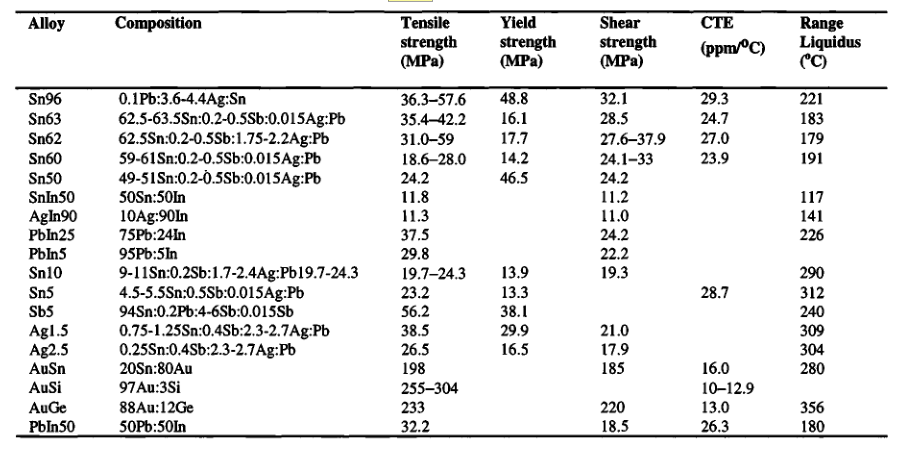
\includegraphics[keepaspectratio, height=.8\textheight, width=\textwidth]{docs/soldes.png}
		\caption{Solders, \cite[p.53]{pecht1998electronic}}
		\label{fig:metals}
	\end{figure}
	
	\begin{figure}[h!]
		\centering
		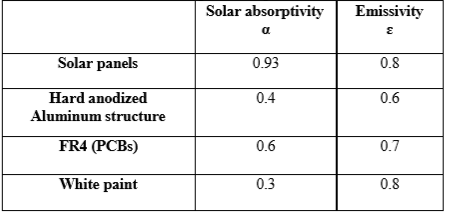
\includegraphics[keepaspectratio, height=.4\textheight, width=\textwidth]{THE/AcubeSAT-THE-BH-032/docs/thermoptic_fr4.png}
		\caption{\cite{ganti2017design}}
		\label{fig:thermoopticfr4}
	\end{figure}
	
	\begin{figure}[h!]
		\centering
		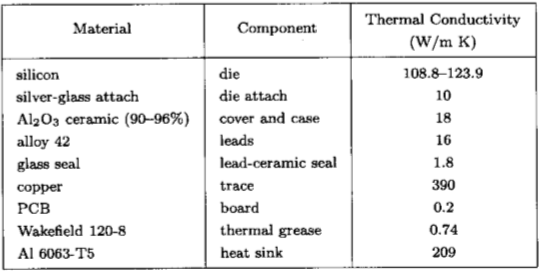
\includegraphics[keepaspectratio, height=.4\textheight, width=\textwidth]{THE/AcubeSAT-THE-BH-032/docs/pcb_properties.png}
		\caption{\cite{teng1997thermal}}
		\label{fig:pcb_level}
	\end{figure}
	
	\begin{figure}[h!]
		\centering
		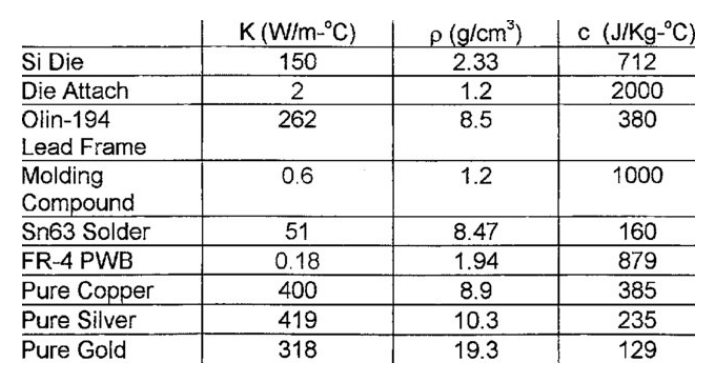
\includegraphics[keepaspectratio, height=.25\textheight, width=\textwidth]{docs/package_properties_no1.png}
		\caption{\cite{kuo1998ic}}
		\label{fig:tab_1}
	\end{figure}
	
	\begin{figure}[h!]
		\centering
		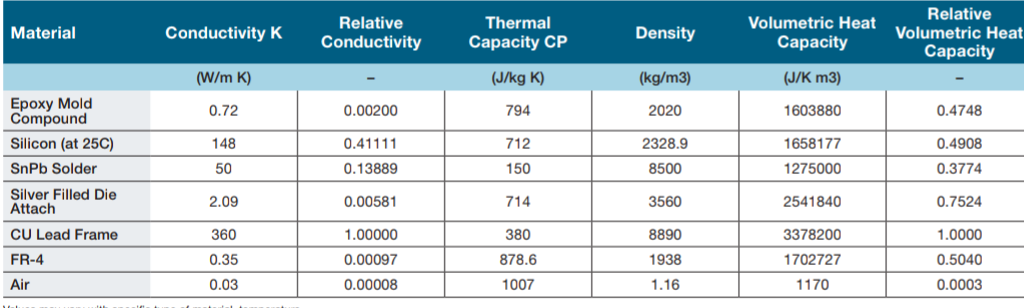
\includegraphics[keepaspectratio, height=.25\textheight, width=\textwidth]{docs/package_properties_no2.png}
		\caption{\cite{nxp:material}}
		\label{fig:tab_2}
	\end{figure}
	
	\begin{figure}[h!]
		\centering
		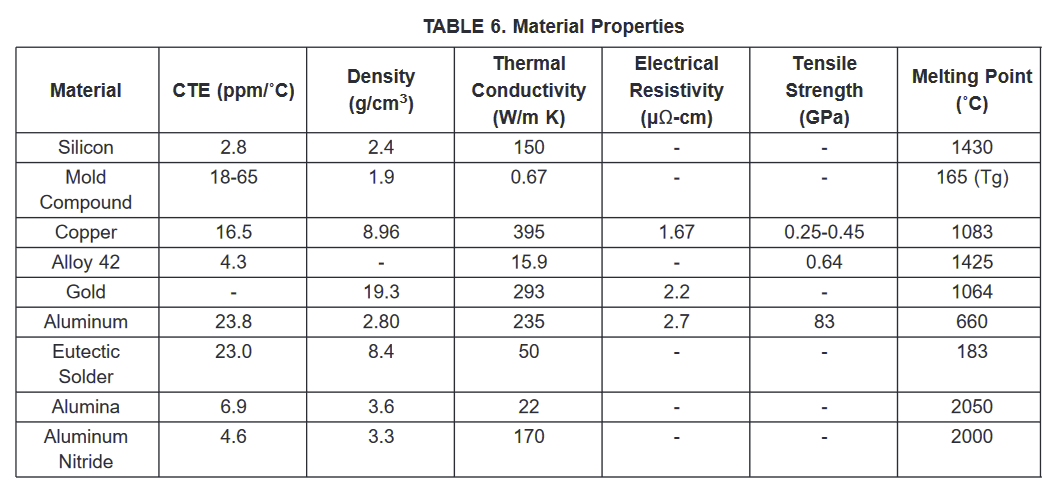
\includegraphics[keepaspectratio, height=.25\textheight, width=\textwidth]{docs/TI_ic_assembly.png}
		\caption{\cite{ti:material}}
		\label{fig:tab_3}
	\end{figure}
	
	\begin{figure}[h!]
		\centering
		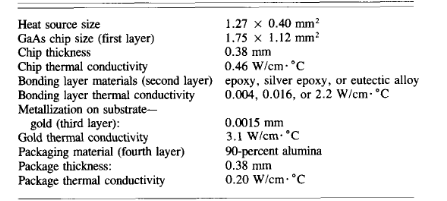
\includegraphics[keepaspectratio, height=.25\textheight, width=\textwidth]{docs/package_properties_no3.png}
		\caption{\cite{49036}}
		\label{fig:tab_4}
	\end{figure}
	
	\begin{figure}[h!]
		\centering
		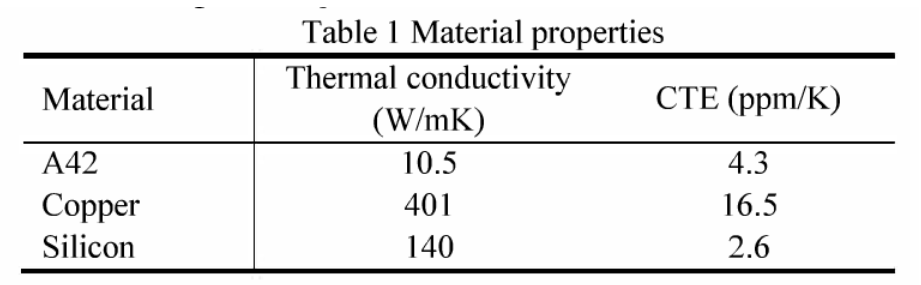
\includegraphics[keepaspectratio, height=.15\textheight, width=\textwidth]{docs/copper_plating_thickness.png}
		\caption{\cite{Li2012EffectsOC}}
		\label{}
	\end{figure}
	
	\clearpage
	
	\bibliographystyle{plain}
	\bibliography{thermal.bib}
	
\end{document}
